% !TEX program = xelatex
\documentclass[10pt,letterpaper,twocolumn]{article}

% === GEOMETRY ===
% Bottom margin + footskip tuned so the page number sits ≥0.6in from the
% sheet edge — clear of consumer-inkjet unprintable zones (HP DeskJet
% bottom dead strip is 0.5in) without scaling the page down.
\usepackage[top=0.75in, bottom=0.75in, left=0.75in, right=0.75in, footskip=12pt]{geometry}

% === FONTS ===
\usepackage{fontspec}
\usepackage{unicode-math}
\setmainfont{Latin Modern Roman}[
 Extension=.otf,
 UprightFont=lmroman10-regular,
 BoldFont=lmroman10-bold,
 ItalicFont=lmroman10-italic,
 BoldItalicFont=lmroman10-bolditalic,
]
\setsansfont{Latin Modern Sans}[
 Extension=.otf,
 UprightFont=lmsans10-regular,
 BoldFont=lmsans10-bold,
 ItalicFont=lmsans10-oblique,
 BoldItalicFont=lmsans10-boldoblique,
]
\setmonofont{Latin Modern Mono}[
 Extension=.otf,
 UprightFont=lmmono10-regular,
 ItalicFont=lmmono10-italic,
 Scale=0.85,
]
% YWFT Processing is used in exactly ONE place: the title in the header.
% Its punctuation glyphs are unreliable (the "/" renders as an ampersand-
% like mark), so body text, subtitle, and the edition slot stay in the
% Latin Modern faces.
\newfontfamily\acbold{ywft-processing-bold}[
 Path=../../system/public/type/webfonts/,
 Extension=.ttf
]

% === PACKAGES ===
\usepackage{xcolor}
\usepackage{colortbl}
\usepackage{titlesec}
\usepackage{enumitem}
\usepackage{booktabs}
\usepackage{tabularx}
\usepackage{fancyhdr}
\usepackage{hyperref}
\usepackage{xurl}
\usepackage{graphicx}
\graphicspath{{./}{figures/}}
\usepackage{ragged2e}
\usepackage{microtype}
\usepackage[font=footnotesize]{caption}
\usepackage{afterpage}
\usepackage{multicol}
\usepackage{natbib}
\usepackage{tikz}
\usetikzlibrary{calc,positioning,shapes.geometric,arrows.meta}

% --- TikZ helpers for inline keyboard / hex / mapping diagrams ---
\definecolor{keyfill}{RGB}{248,248,250}
\definecolor{keystroke}{RGB}{160,156,170}
\definecolor{keymapped}{RGB}{180,72,135}
\definecolor{keysharp}{RGB}{52,52,64}
\tikzset{
 kcap/.style={draw=keystroke, fill=keyfill, rounded corners=0.6pt,
        minimum width=0.34cm, minimum height=0.34cm,
        inner sep=0pt, font=\scriptsize\sffamily},
 kcap mapped/.style={kcap, fill=keymapped!18, draw=keymapped!60,
            text=keymapped!90},
 kcap sharp/.style={kcap, fill=keysharp, draw=keysharp,
           text=white, font=\scriptsize\sffamily\bfseries},
 hexkey/.style={regular polygon, regular polygon sides=6,
         draw=keystroke, fill=keyfill, rounded corners=0pt,
         minimum size=0.55cm, inner sep=0pt,
         font=\tiny\sffamily},
 hexkey mapped/.style={hexkey, fill=keymapped!22, draw=keymapped!70,
             text=keymapped!90},
}
% === COLORS ===
\definecolor{acpink}{RGB}{180,72,135}
\definecolor{acpurple}{RGB}{120,80,180}
\definecolor{acdark}{RGB}{64,56,74}
\definecolor{acgray}{RGB}{119,119,119}
\definecolor{acblue}{RGB}{42,100,212}
\definecolor{acgreen}{RGB}{42,154,58}
\definecolor{acorange}{RGB}{216,120,0}
% Domain chip for the corollary table — small caps-ish bold colored tag
\newcommand{\dmn}[2]{\textcolor{#1}{\textbf{#2}}}
% Row QR code for the corollary table — links each object to its
% canonical home (Wikipedia, the project's own site, or its spec).
% PNGs generated by qrencode + magick PNG32 in figures/qr/.
% Centered on the row's text baseline so label text sits vertically
% centered against the tile.
\newcommand{\qrc}[1]{\raisebox{\dimexpr-0.5\height+0.8ex\relax}{\includegraphics[height=0.74cm]{figures/qr/#1.png}}}

% === HYPERREF ===
\hypersetup{
 colorlinks=true,
 linkcolor=acpurple,
 urlcolor=acpurple,
 citecolor=acpurple,
 pdfauthor={@jeffrey},
 pdftitle={Los mapas de teclado como software social: objetos virtuales versionados mediante contrato social},
}

% === SECTION FORMATTING ===
\titleformat{\section}
 {\normalfont\bfseries\normalsize\uppercase}
 {\thesection.}
 {0.5em}
 {}
\titlespacing{\section}{0pt}{1.2em}{0.3em}

\titleformat{\subsection}
 {\normalfont\bfseries\small}
 {\thesubsection}
 {0.5em}
 {}
\titlespacing{\subsection}{0pt}{0.8em}{0.2em}

% === HEADER/FOOTER ===
\pagestyle{fancy}
\fancyhf{}
\renewcommand{\headrulewidth}{0pt}
\fancyfoot[C]{\footnotesize\thepage}
% Full-page table spread: folio moves to the bottom right so it can't
% collide with the table body.
\fancypagestyle{tablefolio}{%
 \fancyhf{}%
 \renewcommand{\headrulewidth}{0pt}%
 \fancyfoot[R]{\footnotesize\thepage}%
}

% === LIST SETTINGS ===
\setlist[itemize]{nosep, leftmargin=1.2em, itemsep=0.1em}
\setlist[enumerate]{nosep, leftmargin=1.2em}

% === COLUMN SEPARATION ===
\setlength{\columnsep}{1.8em}

% === PARAGRAPH SETTINGS ===
\setlength{\parindent}{1em}
\setlength{\parskip}{0.3em}

% Hyphenation for narrow two-column layout
\tolerance=800
\emergencystretch=1em
\hyphenpenalty=50

\newcommand{\acdot}{{\color{acpink}.}}
% Every dot in Aesthetic.Computer is the AC pink dot, inline too.
\newcommand{\ac}{Aesthetic{\acdot}Computer}
% Keycap chip — the one canonical inline key glyph: cap-height box
% (no descender slack, so it sits low in the text line) with a gray
% bottom-shadow bezel, like the keycaps in the figures.
\DeclareRobustCommand{\key}[1]{\tikz[baseline=(k.base)]{%
 \node[fill=keystroke, rounded corners=1.3pt, inner xsep=2.4pt,
    inner ysep=1.9pt, anchor=base, yshift=-1.2pt] at (0,0)
  {\footnotesize\ttfamily\bfseries\vphantom{A}\phantom{#1}};
 \node[draw=keystroke, line width=0.4pt, fill=keyfill,
    rounded corners=1.3pt, inner xsep=2.4pt, inner ysep=1.9pt,
    anchor=base] (k) at (0,0)
  {\footnotesize\ttfamily\bfseries\vphantom{A}#1};}}
% A run of keycaps with even spacing: \keys{C,D,E,F,G,A,B}
\makeatletter
\DeclareRobustCommand{\keys}[1]{{\def\sep{}\@for\kk:=#1\do{\sep\key{\kk}\def\sep{\,}}}}
\makeatother

% Version stamp (hash + revision). papers/cli.mjs regenerates
% version.tex from git on every build; the fallback defaults keep a
% manual `xelatex keymaps.tex` (no stamp present) compiling.
\InputIfFileExists{version}{}{%
 \providecommand{\paperhash}{dev}\providecommand{\paperrev}{?}}
\InputIfFileExists{history}{}{\providecommand{\paperhistory}{}}

% Cover language bar. The same paper is published in six languages; each
% edition links to the others by their canonical permalink. Language codes
% (not autonyms) keep the row legible in every font --- the Latin-only
% editions cannot render CJK/Cyrillic glyphs. \klanghere marks the current
% language; \klang links a sibling edition by its URL suffix ("" for en).
\newcommand{\klang}[2]{\href{https://papers.aesthetic.computer/keymaps-social-software-26-arxiv#2.pdf}{\color{acgray}#1}}
\newcommand{\klanghere}[1]{{\bfseries\color{acpink}#1}}
\newcommand{\klangsep}{{\color{acgray!60}\,\textperiodcentered\,}}

\begin{document}

\twocolumn[{%
\begin{center}
{\acbold\fontsize{27pt}{31pt}\selectfont\color{acdark} Keymaps as Social Software}\par
\vspace{0.5em}

\includegraphics[width=0.7\textwidth]{figures/cover}\par
\vspace{0.4em}
{\itshape\fontsize{14.5pt}{17pt}\selectfont\color{acpink} Objetos virtuales versionados mediante contrato social}\par
\vspace{0.5em}
{\small\color{acgray} \href{https://prompt.ac/@jeffrey}{@jeffrey} \,$\cdot$\, Aesthetic{\acdot}Computer \,$\cdot$\, ORCID \href{https://orcid.org/0009-0007-4460-4913}{0009-0007-4460-4913}}\par
\vspace{0.45em}
{\footnotesize\sffamily\klang{EN}{}\klangsep\klang{DA}{-da}\klangsep\klanghere{ES}\klangsep\klang{ZH}{-zh}\klangsep\klang{JA}{-ja}\klangsep\klang{RU}{-ru}}\par
\vspace{0.55em}
{\color{acpink}\rule{\textwidth}{1.2pt}}
\vspace{0.5em}
\end{center}

\begin{quote}
\small\noindent\textbf{Resumen.}
Un \emph{mapa de teclado} (keymap) --- la pequeña tabla declarativa que dice ``la tecla QWERTY \key{A} toca el MIDI 60'' --- es software en todo sentido funcional: versionado, inventado, bifurcado y reclamado entre aplicaciones. Pero no es un binario, ni un proyecto, ni un servicio, y el eje código abierto frente a propietario no logra verlo. Nombro la categoría \emph{software social} --- jugando con Shirky y sumándome al uso que le dan McCarthy y Reas en su iniciativa homónima de UCLA, dentro de la cual se escribió este artículo --- y la rastreo desde Sholes hasta Colemak, desde Jankó hasta Wicki--Hayden, y hasta la convención QWERTY-piano sin dueño que distribuye por defecto todo DAW de relevancia --- que denomino el diseño AWSED, por las teclas de sus primeros cinco tonos cromáticos. Leído a través del \emph{Turing Complete User} de Lialina~\citep{lialina2012turing}, el mapa de teclado es la brecha que el usuario puede autorizar y cuya clausura supone la desaparición del usuario como autor; presento el mapa de teclado de \texttt{notepat.com} --- ``notas que se nombran a sí mismas'' --- como prueba de que la brecha sigue abierta.
\end{quote}
\vspace{0.5em}
}]

\section{Introducción: un artefacto}

La Figura~\ref{fig:notepat-keymap} es un diagrama de una página del mapa de teclado que distribuye \texttt{notepat.com}, un instrumento de teclado cromático dentro de \ac{}. El diagrama muestra un teclado de piano arriba, un teclado QWERTY debajo y líneas punteadas que conectan ambos. El principio que los une es el lema bajo el cual se distribuye el proyecto: \emph{notas que se nombran a sí mismas}. La letra QWERTY \key{C} toca C; \key{D} toca D; \key{E} toca E; y así sucesivamente hasta \key{B}. La octava superior continúa alfabéticamente (\keys{H,I,J,K,L,M,N} para $C_5$ hasta $B_5$). Los sostenidos se ubican una fila por encima de su nota natural cuando es posible, por analogía con las teclas negras del piano (\keys{V,S,W,R,Q} para $C^\sharp\,D^\sharp\,F^\sharp\,G^\sharp\,A^\sharp$).

\begin{figure*}[t]
\centering
% Native TikZ rendering of the notepat keymap diagram (Figure 1).
% Replaces the slide-pipeline PNG so the figure matches the paper's
% other vector diagrams. Piano keyboard (with the QWERTY letter that
% plays each note) above, QWERTY keyboard below, dashed color-matched
% connectors between the naturals. No hand labels — the hand split is
% carried by the two background tints and the caption.
% Key mapping verified against fedac/native/pieces/notepat.mjs and the
% AC Native screenshot: H I J K L M N = C5..B5 alphabetically (M=A5,
% N=B5), sharps V S W R Q (lower) and T Y U O P (upper).
\begingroup
% --- notepat note colors (from slides/notepat-keymap/template.html) ---
\definecolor{ncc}{HTML}{FF3232}\definecolor{ncd}{HTML}{FFA000}%
\definecolor{nce}{HTML}{FFE600}\definecolor{ncf}{HTML}{32C832}%
\definecolor{ncg}{HTML}{3278FF}\definecolor{nca}{HTML}{8232C8}%
\definecolor{ncb}{HTML}{B450FF}%
\definecolor{nCC}{HTML}{FF2850}\definecolor{nDD}{HTML}{FFB400}%
\definecolor{nEE}{HTML}{FFFF32}\definecolor{nFF}{HTML}{32FF64}%
\definecolor{nGG}{HTML}{32C8FF}\definecolor{nAA}{HTML}{B432FF}%
\definecolor{nBB}{HTML}{FF50FF}%
\definecolor{extbg}{HTML}{FFF4D6}\definecolor{extfg}{HTML}{8A7330}%
\definecolor{extbd}{HTML}{D4C075}%
\definecolor{extbk}{HTML}{5A4818}\definecolor{extbkfg}{HTML}{F8E7A0}%
\definecolor{octbg}{HTML}{F4ECFF}\definecolor{octfg}{HTML}{6B3FC0}%
\definecolor{octbd}{HTML}{B89DF0}%
\resizebox{\textwidth}{!}{%
\begin{tikzpicture}
% --- geometry ---
% piano: 17 white keys, pitch 1.02, key 0.98 x [4.4 .. 7.5]
% qwerty: caps 0.95, pitch 1.0, rows at y = 2.30 / 1.15 / 0
\def\pw{1.02}
\def\qx{2.45}
% --- piano key macros ---
\def\pkey#1#2#3#4{\begin{scope}[shift={({#1*\pw},0)}]
  \draw[acdark, fill=white, line width=0.8pt, rounded corners=1.5pt]
    (0,4.4) rectangle (0.98,7.5);
  \fill[#4] (0.04,4.44) rectangle (0.94,4.86);
  \draw[acdark!45, line width=0.4pt] (0.04,4.86) -- (0.94,4.86);
  % letter + note name live in the band BELOW the black keys
  \node[font=\large\ttfamily\bfseries, text=acdark] at (0.49,5.34) {#2};
  \node[font=\scriptsize\ttfamily, text=acdark!80] at (0.49,5.02) {#3};
\end{scope}}
\def\pkeyext#1#2#3{\begin{scope}[shift={({#1*\pw},0)}]
  \draw[extbd, dashed, fill=extbg, fill opacity=0.55, line width=0.8pt, rounded corners=1.5pt]
    (0,4.4) rectangle (0.98,7.5);
  \node[font=\large\ttfamily\bfseries, text=extfg, opacity=0.75] at (0.49,5.34) {#2};
  \node[font=\scriptsize\ttfamily, text=extfg, opacity=0.75] at (0.49,5.02) {#3};
\end{scope}}
\def\pbkey#1#2#3{\begin{scope}[shift={({#1},0)}]
  \draw[black, fill=black!92, line width=0.8pt, rounded corners=1.2pt]
    (-0.31,5.55) rectangle (0.31,7.5);
  \node[font=\normalsize\ttfamily\bfseries, text=white] at (0,6.98) {#2};
  \node[font=\fontsize{5.5pt}{5.5pt}\selectfont\ttfamily, text=white!75!black]
    at (0,6.45) {#3};
\end{scope}}
\def\pbkeyext#1#2#3{\begin{scope}[shift={({#1},0)}]
  \draw[extbk!80!black, dashed, fill=extbk, fill opacity=0.55, line width=0.8pt, rounded corners=1.2pt]
    (-0.31,5.55) rectangle (0.31,7.5);
  \node[font=\normalsize\ttfamily\bfseries, text=extbkfg, opacity=0.8] at (0,6.98) {#2};
  \node[font=\fontsize{5.5pt}{5.5pt}\selectfont\ttfamily, text=extbkfg!80]
    at (0,6.45) {#3};
\end{scope}}
% --- qwerty cap macros ---
% mapped natural: colored fill; #5 = label color (white or dark)
\def\qcap#1#2#3#4#5#6{\begin{scope}[shift={({#1},{#2})}]
  \draw[#4, fill=#3, line width=1pt, rounded corners=2.2pt]
    (0,0) rectangle (0.95,0.95);
  \node[font=\large\ttfamily\bfseries, text=#5] at (0.475,0.475) {\strut#6};
\end{scope}}
% sharp: near-black cap, border in the sharp's note color
\def\qsharp#1#2#3#4{\begin{scope}[shift={({#1},{#2})}]
  \draw[#3, fill=black!90, line width=1.1pt, rounded corners=2.2pt]
    (0,0) rectangle (0.95,0.95);
  \node[font=\large\ttfamily\bfseries, text=white] at (0.475,0.475) {\strut#4};
\end{scope}}
\def\qext#1#2#3{\begin{scope}[shift={({#1},{#2})}]
  \draw[extbd, dashed, fill=extbg, fill opacity=0.55, line width=1pt, rounded corners=2.2pt]
    (0,0) rectangle (0.95,0.95);
  \node[font=\large\ttfamily\bfseries, text=extfg, opacity=0.75] at (0.475,0.475) {\strut#3};
\end{scope}}
\def\qextbk#1#2#3{\begin{scope}[shift={({#1},{#2})}]
  \draw[extbk!80!black, dashed, fill=extbk, fill opacity=0.55, line width=1pt, rounded corners=2.2pt]
    (0,0) rectangle (0.95,0.95);
  \node[font=\large\ttfamily\bfseries, text=extbkfg, opacity=0.75] at (0.475,0.475) {\strut#3};
\end{scope}}
\def\qghost#1#2#3{\begin{scope}[shift={({#1},{#2})}]
  \draw[black!22, dashed, line width=0.9pt, rounded corners=2.2pt]
    (0,0) rectangle (0.95,0.95);
  \node[font=\large\ttfamily, text=black!30] at (0.475,0.475) {\strut#3};
\end{scope}}
\def\qoct#1#2#3#4{\begin{scope}[shift={({#1},{#2})}]
  \draw[octbd, fill=octbg, line width=1pt, rounded corners=2.2pt]
    (0,0) rectangle (0.95,0.95);
  \node[font=\large\ttfamily\bfseries, text=octfg] at (0.475,0.55) {\strut#3};
  \node[font=\fontsize{5pt}{5pt}\selectfont\sffamily\bfseries, text=octfg!75]
    at (0.475,0.2) {#4};
\end{scope}}
% --- hand-split background tints behind the qwerty block ---
\fill[acblue!8, rounded corners=4pt] (\qx-0.25,-0.3) rectangle (\qx+6.07,3.55);
\fill[acpink!8, rounded corners=4pt] (\qx+6.07,-0.3) rectangle (\qx+12.6,3.55);
% --- connectors (drawn LAST so they compose over the keys) ---
\def\conn#1#2#3#4#5{%
  \draw[#4, dashed, line width=1.1pt, opacity=#5, line cap=round]
    ({#1*\pw+0.49},4.62) -- ({#2+0.475},{#3+0.80});
  \fill[#4, opacity=#5] ({#1*\pw+0.49},4.62) circle (0.055);
  \fill[#4, opacity=#5] ({#2+0.475},{#3+0.80}) circle (0.055);}
% --- piano: white keys ---
\pkeyext{0}{X}{B3}
\pkey{1}{C}{C4}{ncc}  \pkey{2}{D}{D4}{ncd}  \pkey{3}{E}{E4}{nce}
\pkey{4}{F}{F4}{ncf}  \pkey{5}{G}{G4}{ncg}  \pkey{6}{A}{A4}{nca}
\pkey{7}{B}{B4}{ncb}
\pkey{8}{H}{C5}{nCC}  \pkey{9}{I}{D5}{nDD}  \pkey{10}{J}{E5}{nEE}
\pkey{11}{K}{F5}{nFF} \pkey{12}{L}{G5}{nGG} \pkey{13}{M}{A5}{nAA}
\pkey{14}{N}{B5}{nBB}
\pkeyext{15}{;}{C6} \pkeyext{16}{]}{D6}
% --- piano: black keys (centered on white-key boundaries) ---
\pbkeyext{0.35}{Z}{A\#3}
\pbkey{2.04}{V}{C\#4}  \pbkey{3.06}{S}{D\#4}
\pbkey{5.10}{W}{F\#4}  \pbkey{6.12}{R}{G\#4}  \pbkey{7.14}{Q}{A\#4}
\pbkey{9.18}{T}{C\#5}  \pbkey{10.20}{Y}{D\#5}
\pbkey{12.24}{U}{F\#5} \pbkey{13.26}{O}{G\#5} \pbkey{14.28}{P}{A\#5}
\pbkeyext{16.32}{'}{C\#6}
% --- qwerty row 0 (top): Q W E R T Y U I O P [ ] ---
\qsharp{\qx+0}{2.30}{nca}{Q}
\qsharp{\qx+1}{2.30}{ncf}{W}
\qcap{\qx+2}{2.30}{nce}{nce!60!black}{black!75}{E}
\qsharp{\qx+3}{2.30}{ncg}{R}
\qsharp{\qx+4}{2.30}{nCC}{T}
\qsharp{\qx+5}{2.30}{nDD}{Y}
\qsharp{\qx+6}{2.30}{nFF}{U}
\qcap{\qx+7}{2.30}{nDD}{nDD!60!black}{white}{I}
\qsharp{\qx+8}{2.30}{nGG}{O}
\qsharp{\qx+9}{2.30}{nAA}{P}
\qghost{\qx+10}{2.30}{[}
\qext{\qx+11}{2.30}{]}
% --- qwerty row 1 (home): A S D F G H J K L ; ' ---
\qcap{\qx+0.28+0}{1.15}{nca}{nca!60!black}{white}{A}
\qsharp{\qx+0.28+1}{1.15}{ncd}{S}
\qcap{\qx+0.28+2}{1.15}{ncd}{ncd!60!black}{white}{D}
\qcap{\qx+0.28+3}{1.15}{ncf}{ncf!60!black}{white}{F}
\qcap{\qx+0.28+4}{1.15}{ncg}{ncg!60!black}{white}{G}
\qcap{\qx+0.28+5}{1.15}{nCC}{nCC!60!black}{white}{H}
\qcap{\qx+0.28+6}{1.15}{nEE}{nEE!55!black}{black!70}{J}
\qcap{\qx+0.28+7}{1.15}{nFF}{nFF!55!black}{black!60}{K}
\qcap{\qx+0.28+8}{1.15}{nGG}{nGG!55!black}{black!60}{L}
\qext{\qx+0.28+9}{1.15}{;}
\qextbk{\qx+0.28+10}{1.15}{'}
% --- qwerty row 2 (bottom): Z X C V B N M , . / ---
\qextbk{\qx+0.84+0}{0}{Z}
\qext{\qx+0.84+1}{0}{X}
\qcap{\qx+0.84+2}{0}{ncc}{ncc!60!black}{white}{C}
\qsharp{\qx+0.84+3}{0}{ncc}{V}
\qcap{\qx+0.84+4}{0}{ncb}{ncb!60!black}{white}{B}
\qcap{\qx+0.84+5}{0}{nBB}{nBB!60!black}{white}{N}
\qcap{\qx+0.84+6}{0}{nAA}{nAA!60!black}{white}{M}
\qoct{\qx+0.84+7}{0}{,}{OCT$-$}
\qoct{\qx+0.84+8}{0}{.}{OCT$+$}
\qghost{\qx+0.84+9}{0}{/}
% connectors drawn last — composed over the keys
\conn{1}{\qx+0.84+2}{0}{ncc}{0.85}      % C4 -> C (row 2)
\conn{2}{\qx+0.28+2}{1.15}{ncd}{0.65}   % D4 -> D
\conn{3}{\qx+2}{2.30}{nce!75!black}{0.55} % E4 -> E
\conn{4}{\qx+0.28+3}{1.15}{ncf}{0.50}   % F4 -> F
\conn{5}{\qx+0.28+4}{1.15}{ncg}{0.45}   % G4 -> G
\conn{6}{\qx+0.28+0}{1.15}{nca}{0.40}   % A4 -> A
\conn{7}{\qx+0.84+4}{0}{ncb}{0.35}      % B4 -> B
\conn{8}{\qx+0.28+5}{1.15}{nCC}{0.55}   % C5 -> H
\conn{9}{\qx+7}{2.30}{nDD}{0.45}        % D5 -> I
\conn{10}{\qx+0.28+6}{1.15}{nEE!70!black}{0.40} % E5 -> J
\conn{11}{\qx+0.28+7}{1.15}{nFF!80!black}{0.40} % F5 -> K
\conn{12}{\qx+0.28+8}{1.15}{nGG!80!black}{0.40} % G5 -> L
\conn{13}{\qx+0.84+6}{0}{nAA}{0.35}     % A5 -> M
\conn{14}{\qx+0.84+5}{0}{nBB}{0.32}     % B5 -> N
\end{tikzpicture}}
\endgroup

\caption{El mapa de teclado de \texttt{notepat.com}. La letra QWERTY \key{C} toca C, \key{D} toca D, ..., \key{B} toca B; la octava superior continúa alfabéticamente (\keys{H,I,J,K,L,M,N}); los sostenidos se ubican por encima de su nota natural por analogía con las teclas negras del piano cuando es posible. División a dos manos: la octava inferior bajo la mano izquierda (campo azul), la superior bajo la derecha (campo rosa); las teclas atenuadas amplían el registro. Implementaciones: \texttt{notepat.com} (web), AC Native OS, MenuBand (barra de menús de macOS), complemento de Ableton (Max for Live), \texttt{babypat}.}
\label{fig:notepat-keymap}
\end{figure*}

Este diagrama es el artefacto. Es pequeño. No contiene código. No es un binario, ni un servicio, ni un entorno de ejecución. Es una tabla. Y sin embargo, de todos los componentes que constituyen \texttt{notepat.com}, la tabla es la que viaja --- la que cualquiera que toque un instrumento derivado de notepat a través de la web, AC Native, la barra de menús de macOS, Max for Live o la aplicación de teléfono debe conocer y aceptar. La tabla es lo que hace que \texttt{notepat.com} sea \emph{él mismo} a través de los sustratos --- y lo mismo vale para los instrumentos en general: el mapa de teclado es lo que da a un instrumento, \texttt{notepat.com} o cualquier otro, su identidad en cada superficie que lo alberga.

Este artículo trata sobre ese tipo de tabla. La llamaré \emph{mapa de teclado}, y argumentaré que los mapas de teclado forman una categoría de artefacto computacional que el marco habitual de la academia informática --- un marco organizado en torno a binarios, proyectos y licencias --- no logra ver. La categoría no es pequeña. Entre sus otros miembros se cuentan el propio diseño QWERTY, el diseño Dvorak, Colemak y sus bifurcaciones, el diseño de notas isomórfico Wicki--Hayden, la asignación cromática en escalera QWERTY-piano que comparte todo DAW de relevancia, la notación Singmaster para algoritmos del cubo de Rubik~\citep{singmaster1981notes}, el Nashville Number System~\citep{matthews1984nashville}, la teoría estenográfica de Plover~\citep{knight2010plover}, la notación de pad numérico de los juegos de lucha, la Rueda Camelot~\citep{davis1991camelot} y las combinaciones de teclas de Vim, entre muchos otros.

Llamaré a la categoría \emph{software social}, y el nombre arrastra dos linajes a la vez. El primero es el término de Shirky de 2003~\citep{shirky2003etech,allen2004socialsoftware}: donde Shirky y sus contemporáneos usaron ``software social'' para designar \emph{software que media la interacción social} --- foros, wikis, sistemas de chat --- yo lo uso para designar \emph{software cuya existencia \textbf{es} un acuerdo social}. Esa lectura es un juego de palabras, paralelo y un poco sorprendente. El segundo linaje está más cerca, y es el contexto dentro del cual se escribió este artículo: \emph{Social Software} es la iniciativa de UCLA Design\,\textbar\,Media Arts dirigida por Lauren Lee McCarthy y Casey Reas~\citep{sosoft_info}, que define su objeto como ``cualquier sistema que organiza el comportamiento, coordina a las personas o estructura la interacción'' --- \emph{Auto} de McCarthy, una performance escenificada dentro de un vehículo autónomo, es software social precisamente en ese sentido~\citep{mccarthy2026auto}. Escribo como artista en residencia en el segundo ciclo de la iniciativa, \emph{Scores for Social Software}, dirigido por Reas~\citep{reas2026scores}, que lee la \emph{partitura} (score) --- la instrucción Fluxus, las \emph{Notations} de Cage y Knowles, el \emph{do it} de Obrist~\citep{cage1969notations,obrist1997doit} --- como una forma de coreografiar acontecimientos en el tiempo mediante texto, diagramas u otras formas de instrucción. Un mapa de teclado es precisamente una partitura de ese tipo: una pequeña tabla instructiva que coreografía las manos, se propaga como texto y diagrama, y organiza el comportamiento de todos los que la adoptan. Un mapa de teclado no tiene compilador, ni entorno de ejecución, ni organización que lo mantenga, y rara vez un mecanismo financiero que lo respalde. Existe porque suficientes personas decidieron actuar como si existiera. Persiste porque los usuarios exigen compatibilidad con él a través de los binarios. Cuando esa compatibilidad se rompe, los usuarios lo notan; cuando se preserva, el mapa de teclado se propaga aún más.

El artículo avanza en siete movimientos. \textsection\ref{sec:category} plantea el problema de la categoría: los mapas de teclado tienen forma de software pero no son software, y el eje código abierto/propietario no logra verlos. \textsection\ref{sec:lineage1}--\ref{sec:lineage2} rastrean dos linajes de invención de mapas de teclado --- el linaje de la máquina de escribir al ordenador (Sholes, Dvorak, Colemak) y el linaje del instrumento musical (Janko, Wicki--Hayden, los modernos controladores hexagonales isomórficos). \textsection\ref{sec:daw} examina el caso contemporáneo dominante: el mapa de teclado cromático en escalera QWERTY-piano que Ableton, Logic, GarageBand y FL Studio distribuyen por defecto --- una convención sin dueño que nadie diseñó, nadie mantiene y todos implementan. \textsection\ref{sec:notepat} lee el mapa de teclado ``notas que se nombran a sí mismas'' de \texttt{notepat.com} como una intervención deliberada contra ese titular: no una herencia, ni una bifurcación, sino una propuesta rival sobre cómo debería ser la tabla --- y traza la línea entre el contrato tonal, que toda implementación debe llevar, y la capa de interpretación extendida, que cada sustrato cultiva por su cuenta. \textsection\ref{sec:notation} introduce la superficie de notación: todo mapa de teclado tiene una forma textual en la que viaja su uso, y la notación es a menudo la mitad más duradera del artefacto --- una afirmación estructural con Vim como caso positivo canónico y la escalera cromática de los DAW como el negativo. \textsection\ref{sec:corollaries} cataloga el género más amplio, mostrando que las asignaciones de entrada, los sistemas de notación y las etiquetas de categoría comparten un patrón común de software social. \textsection\ref{sec:lialina} lee el cuerpo de pruebas a través del \emph{Turing Complete User} de Lialina, argumentando que los mapas de teclado son el cuerpo empírico de su afirmación de que los usuarios son programadores en espera. \textsection\ref{sec:design} cierra con lo que esto exige a los diseñadores: distribuir el mapa de teclado como un objeto de primera clase --- legible, exportable, bifurcable --- y la notación junto a él.

\section{El problema de la categoría}
\label{sec:category}

Un mapa de teclado es una pequeña tabla declarativa. Su forma mínima es una lista de pares: \emph{(evento-de-tecla-física, salida-semántica)}. El diseño QWERTY es la tabla que empareja posiciones de teclas con letras; el diseño Dvorak reasigna las mismas posiciones a un conjunto distinto de letras; la asignación cromática en escalera QWERTY-piano empareja cada tecla con un número de nota MIDI; la notación de cubo de Singmaster empareja cada etiqueta de cara con un operador de rotación. En todos los casos, la tabla es el artefacto. El binario que consume la tabla es intercambiable.

Esto hace que los mapas de teclado sean difíciles de ubicar dentro de los marcos predominantes de la academia informática. El eje código abierto/propietario~\citep{galloway2004protocol} clasifica el software por el estatus legal de su código fuente. Un mapa de teclado no tiene fuente --- es una tabla, no un programa. El eje de los estudios de plataforma~\citep{nieborg2018platformization} clasifica el software por la plataforma sobre la que se asienta. Un mapa de teclado se asienta sobre \emph{cada} plataforma que consume su forma. El eje de la teoría de formatos~\citep{sterne2012mp3} clasifica el software por la especificación que implementa. Un mapa de teclado rara vez tiene especificación; la asignación cromática en escalera QWERTY-piano no tiene ninguna, y sin embargo cuatro de los mayores DAW del mundo distribuyen todos la misma. El eje de los protocolos~\citep{galloway2004protocol} clasifica el software por el formato de cable que habla. Un mapa de teclado no es un formato de cable; es una tabla consultada en el límite de la entrada.

\emph{MP3: The Meaning of a Format} de Sterne~\citep{sterne2012mp3} es lo que más se acerca. Sterne sostiene que ``los formatos, los estándares y las infraestructuras --- y la necesidad de que el contenido encaje dentro de ellos --- son tan centrales para la comunicación como las cajas que llamamos `medios'.'' Sustitúyase \emph{formato} por \emph{mapa de teclado} y la mayor parte de su aparato se traslada sin problema. Pero los formatos tienen especificaciones (RFC, documentos ISO, implementaciones de referencia). Los mapas de teclado por lo general no. La asignación cromática en escalera QWERTY-piano está implementada en Ableton Live, Logic Pro, GarageBand y FL Studio~\citep{ableton_musical_typing,apple_logic_musicaltyping,imageline_typing_piano} sin haber sido jamás consignada en una especificación vinculante. Existe porque las cuatro implementaciones coinciden, y las cuatro implementaciones coinciden porque todo el que aprendió una espera que la siguiente sea igual.

\emph{Sorting Things Out} de Bowker y Star~\citep{bowker1999sorting} trata las clasificaciones y los estándares como objetos sociopolíticos cuya persistencia es sociológica, no técnica. Un mapa de teclado es una clasificación: ordena las entradas físicas en categorías semánticas. El \emph{objeto frontera} (boundary object) de Star y Griesemer~\citep{star1989boundary} captura otro aspecto: los mapas de teclado median entre comunidades de práctica (mecanógrafo y programador; pianista y usuario de DAW; cubero y resolutor de cubos) sin pertenecer del todo a ninguna. La \emph{etnografía de la infraestructura} de Star~\citep{star1999ethnography} captura un tercero: los mapas de teclado son aburridos, consecuentes y en gran medida invisibles para quienes dependen de ellos.

Lo que queremos nombrar es la conjunción de estos rasgos: una pequeña tabla que es una clasificación (Bowker \& Star), un objeto frontera (Star \& Griesemer), una infraestructura (Star) y un formato (Sterne) --- pero que no es ninguna de esas cosas por sí sola. Propongo \emph{software social} para la conjunción. El término arrastra ahora tres lecturas, y todas son reales. En 2003 nombró \emph{software para la sociabilidad} (Shirky); en UCLA hoy nombra \emph{cualquier sistema que organiza el comportamiento, coordina a las personas o estructura la interacción} (McCarthy y Reas~\citep{sosoft_info}); este artículo propone que también nombre \emph{software de acuerdo social}. Un mapa de teclado es la tercera lectura sin más --- y, leído como una partitura que coreografía las manos de todos los que la adoptan, se sitúa de lleno dentro de la segunda.

\section{Linaje I: diseños de teclado}
\label{sec:lineage1}

El ejemplo sostenido más temprano de un mapa de teclado como software social es el propio diseño QWERTY. Christopher Latham Sholes patentó una máquina de escribir temprana junto con Carlos Glidden y Samuel Soulé en 1868 (US 79{,}265); la disposición QWERTY tal como se distribuyó fue finalizada de forma interna por los mecánicos de Remington en la primavera y el verano de 1873 como una decisión de ingeniería de fabricación, y \emph{nunca se patentó}~\citep{yasuoka2011prehistory}. El relato folclórico habitual atribuye el diseño a una mecánica antiatasco; el trabajo de archivo de Yasuoka y Yasuoka lo localiza en la práctica de transcripción de los operadores de telégrafo, que necesitaban teclear código Morse en tiempo real. En cualquier caso, la persistencia del diseño es sociológica: es el caso empírico fundacional de la economía de la dependencia de la trayectoria~\citep{david1985qwerty,arthur1989competing}, con una contracorriente que sostiene que el dominio se ha exagerado~\citep{liebowitz1990fable}. La disputa David--Liebowitz es la escena primigenia para tratar una asignación de entrada como un objeto cuya persistencia es una cuestión empírica sobre la adopción social, más que una consecuencia derivable de la superioridad técnica.

August Dvorak y William Dealey patentaron el Dvorak Simplified Keyboard en 1936 (US 2{,}040{,}248). Afirmaban que era más rápido, menos fatigante y más racional desde el punto de vista pedagógico que QWERTY. Se propagó de forma desigual: la Marina de EE.\,UU.\ lo adoptó en estudios durante la Segunda Guerra Mundial; el Apple IIc incorporó un conmutador Dvorak; los sistemas operativos modernos distribuyen todos Dvorak como un diseño seleccionable; y una comunidad pequeña pero perdurable de usuarios lo ha utilizado durante décadas. Workman~\citep{bucao2010workman}, Colemak~\citep{coleman2006colemak} y el ecosistema de bifurcaciones posterior a 2010 (Colemak-DH, Halmak, Norman) constituyen una tercera generación. Ninguno de estos diseños tiene una organización que lo mantenga. Ninguno tiene ingresos. Todos son objetos virtuales versionados que se propagan a través de foros, repositorios de GitHub y archivos de diseño de los sistemas operativos. El teclado Maltron~\citep{malt1977keyboard} añadió una variante acoplada al hardware; la teoría estenográfica de Plover~\citep{knight2010plover} extendió la superficie para abarcar la taquigrafía acordada. Los diseños nacionales (AZERTY, QWERTZ, BÉPO) participan de la misma lógica, con el giro adicional del reconocimiento estatal formal: el diseño francés BÉPO, diseñado por una comunidad en 2005, fue incorporado a una norma nacional AFNOR de 2019 --- una transición literalmente observable de contrato social a contrato estatal.

\begin{figure}[t]
\centering
\resizebox{\columnwidth}{!}{%
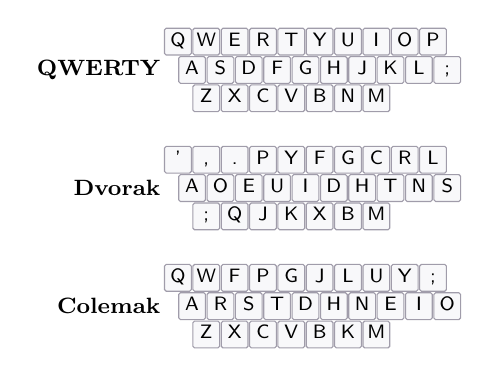
\begin{tikzpicture}
% Three keyboards stacked. Same 30 physical key positions; each layout
% reassigns the letters at those positions. Visual comparison highlights
% how a keymap is a re-binding of an unchanged physical substrate.
% Three keyboards stacked. Punctuation chars are wrapped in {} so
% TikZ's \foreach parser doesn't treat them as separators.
\foreach \layoutY/\name in {3.0/QWERTY, 1.5/Dvorak, 0.0/Colemak} {
 \node[anchor=east, font=\footnotesize\bfseries] at (-0.1, \layoutY+0.36) {\name};
}
% QWERTY rows
\foreach \l [count=\i] in {Q,W,E,R,T,Y,U,I,O,P}
 \node[kcap] at ({(\i-1)*0.36}, 3.72) {\strut\l};
\foreach \l [count=\i] in {A,S,D,F,G,H,J,K,L,{;}}
 \node[kcap] at ({(\i-1)*0.36+0.18}, 3.36) {\strut\l};
\foreach \l [count=\i] in {Z,X,C,V,B,N,M}
 \node[kcap] at ({(\i-1)*0.36+0.36}, 3.0) {\strut\l};
% Dvorak rows
\foreach \l [count=\i] in {{'},{,},{.},P,Y,F,G,C,R,L}
 \node[kcap] at ({(\i-1)*0.36}, 2.22) {\strut\l};
\foreach \l [count=\i] in {A,O,E,U,I,D,H,T,N,S}
 \node[kcap] at ({(\i-1)*0.36+0.18}, 1.86) {\strut\l};
\foreach \l [count=\i] in {{;},Q,J,K,X,B,M}
 \node[kcap] at ({(\i-1)*0.36+0.36}, 1.5) {\strut\l};
% Colemak rows
\foreach \l [count=\i] in {Q,W,F,P,G,J,L,U,Y,{;}}
 \node[kcap] at ({(\i-1)*0.36}, 0.72) {\strut\l};
\foreach \l [count=\i] in {A,R,S,T,D,H,N,E,I,O}
 \node[kcap] at ({(\i-1)*0.36+0.18}, 0.36) {\strut\l};
\foreach \l [count=\i] in {Z,X,C,V,B,K,M}
 \node[kcap] at ({(\i-1)*0.36+0.36}, 0) {\strut\l};
\end{tikzpicture}}
\caption{Tres mapas de teclado de escritura sobre el mismo sustrato físico. Cada diseño es una reasignación de posiciones de teclas idénticas a un conjunto distinto de letras. QWERTY (Sholes 1873, nunca patentado), Dvorak (Dvorak \& Dealey 1936, US 2{,}040{,}248), Colemak (Coleman 2006, dominio público). El ecosistema de bifurcaciones posterior a 2010 prolonga esta línea.}
\label{fig:typing-layouts}
\end{figure}

\section{Linaje II: diseños de instrumento}
\label{sec:lineage2}

Los diseños de instrumentos musicales han recorrido una historia paralela. El teclado de piano isomórfico de seis filas de Paul von Jankó~\citep{janko1882} fue respaldado por Liszt y Rubinstein, fabricado por Decker, Blüthner y Bösendorfer, y enseñado en un Janko Conservatory de Nueva York. Por toda precondición social para la adopción debería haber reemplazado al teclado de piano estándar. No lo hizo. Se sabe que sobreviven menos de diez pianos Janko. El caso Janko es el polo negativo del argumento del mapa de teclado como software social: se cumplieron todas las condiciones para la propagación y la propagación aun así fracasó. Sea cual sea el contrato del software social, es más que la suma de respaldos, fabricantes y conservatorios.

El teclado generalizado de R.\ H.\ M.\ Bosanquet~\citep{bosanquet1875generalized} fue un armonio enarmónico de 53 divisiones iguales de la octava (53-EDO) y un órgano de 1875 en temperamento mesotónico esquismático y de coma de un cuarto de 48 notas, demostrado en el South Kensington Museum en 1876. Es el ancestro de prácticamente todo controlador isomórfico moderno. Kaspar Wicki patentó un diseño de notas isomórfico para bandoneón en 1896~\citep{wicki1896}; Brian Hayden, un intérprete de concertina, reinventó y volvió a patentar de forma independiente esencialmente el mismo diseño en 1986. La doble invención con noventa años de diferencia es en sí misma un argumento: el diseño tiene el carácter de un \emph{descubrimiento}, el tipo de objeto que recurre porque la estructura subyacente de la música lo hace útil, no porque sea un artefacto cultural único.

\begin{figure}[t]
\centering
\resizebox{0.88\columnwidth}{!}{%
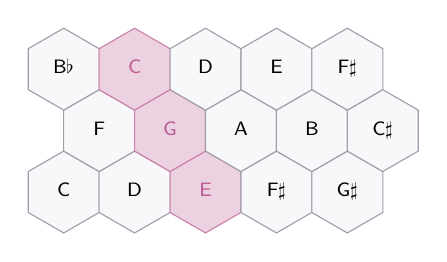
\begin{tikzpicture}
% Compact Wicki-Hayden-style hex schematic. Same-row neighbors
% differ by a whole tone; up-and-right neighbors differ by a P4.
% C major triad (C-E-G) highlighted; the same shape transposes to
% any key by translation across the surface ("isomorphism" claim).
% Hexes are EXPLICIT PATHS, not regular-polygon nodes — TikZ node
% sizing breaks the lattice. Pointy-top hexagon, circumradius R:
% width = sqrt(3)R, height = 2R. Tessellation: horizontal pitch =
% sqrt(3)R, row step = 1.5R, odd-row offset = sqrt(3)R/2.
\def\R{0.52}
\def\hexn#1#2#3{\begin{scope}[shift={(#1,#2)}]
 \draw[keystroke, fill=keyfill]
  (30:\R) -- (90:\R) -- (150:\R) -- (210:\R) -- (270:\R) -- (330:\R) -- cycle;
 \node[font=\scriptsize\sffamily, inner sep=0pt] at (0,0) {\strut#3};
\end{scope}}
\def\hexm#1#2#3{\begin{scope}[shift={(#1,#2)}]
 \draw[keymapped!70, fill=keymapped!25]
  (30:\R) -- (90:\R) -- (150:\R) -- (210:\R) -- (270:\R) -- (330:\R) -- cycle;
 \node[font=\scriptsize\sffamily, text=keymapped!90, inner sep=0pt] at (0,0) {\strut#3};
\end{scope}}
\def\hp{0.9006}  % horizontal pitch (sqrt(3) * R)
\def\vp{0.78}   % vertical pitch (1.5 * R)
\def\offx{0.4503} % horizontal offset for alternate rows (hp / 2)
% Row 0 (bottom)
\hexn{0}{0}{C}
\hexn{\hp}{0}{D}
\hexm{2*\hp}{0}{E}
\hexn{3*\hp}{0}{F$\sharp$}
\hexn{4*\hp}{0}{G$\sharp$}
% Row 1 (middle, offset)
\hexn{\offx}{\vp}{F}
\hexm{\offx + \hp}{\vp}{G}
\hexn{\offx + 2*\hp}{\vp}{A}
\hexn{\offx + 3*\hp}{\vp}{B}
\hexn{\offx + 4*\hp}{\vp}{C$\sharp$}
% Row 2 (top)
\hexn{0}{2*\vp}{B$\flat$}
\hexm{\hp}{2*\vp}{C}
\hexn{2*\hp}{2*\vp}{D}
\hexn{3*\hp}{2*\vp}{E}
\hexn{4*\hp}{2*\vp}{F$\sharp$}
\end{tikzpicture}}
\caption{Diseño hexagonal Wicki--Hayden (Wicki 1896 / Hayden 1986). Los vecinos de la misma fila difieren en un tono entero; los vecinos hacia arriba y a la derecha, en una cuarta justa. La tríada de Do mayor ($C\,E\,G$) está resaltada: el acorde es una forma fija de tres celdas sobre la superficie, y trasladar esa forma transpone el acorde a cualquier tonalidad. ``Transponer es trasladar'' es la afirmación central del teclado isomórfico, y la propiedad que la asimetría de blancas y negras del piano estándar sacrifica.}
\label{fig:wicki}
\end{figure}

\begin{figure*}[t]
\centering
% Interval-signature bars (full text width). Each bar reads left to
% right as the sequence of intervals the instrument's layout steps
% through; every block is one interval, its WIDTH = its size in
% semitones and its COLOR fixed by the legend. A regular instrument
% is a row of equal blocks; an asymmetric one has a visible odd block.
\begingroup
\definecolor{iv1}{HTML}{E2574C}% m2 (1 semitone)
\definecolor{iv2}{HTML}{EE9B3A}% M2 (2)
\definecolor{iv3}{HTML}{D1A52A}% m3 (3) — darkened so white slice text reads
\definecolor{iv4}{HTML}{4FAE54}% M3 (4)
\definecolor{iv5}{HTML}{3A86D6}% P4 (5)
\definecolor{iv7}{HTML}{8A5CF6}% P5 (7)
\resizebox{\textwidth}{!}{%
\begin{tikzpicture}
\def\rad{1.55}
% \pie{xshift}{name}{deg-per-semitone}{ semitones/color/label, ... }
% Slices sweep clockwise from 12 o'clock; angle = semitones. A regular
% instrument is an even wheel; an asymmetric one has a visibly odd slice.
% list fields: semitones / fill / interval-label / note-label.
% The note sits INSIDE the slice (the actual open string, scale degree,
% or valve number); the interval name sits just outside the rim.
\def\pie#1#2#3#4{\begin{scope}[shift={(#1,0)}]
 \xdef\angA{90}
 \foreach \s/\c/\lab/\nt in {#4}{
  \pgfmathsetmacro\angB{\angA-\s*#3}
  \filldraw[fill=\c, draw=\c!55!black, line width=0.6pt]
   (0,0) -- (\angA:\rad) arc[start angle=\angA, end angle=\angB, radius=\rad] -- cycle;
  \pgfmathsetmacro\angM{(\angA+\angB)/2}
  \node[font=\large\sffamily\bfseries, text=white] at (\angM:{0.58*\rad}) {\nt};
  \node[font=\small\sffamily, text=acdark] at (\angM:{\rad+0.32}) {\lab};
  \xdef\angA{\angB}
 }
 \node[font=\normalsize\sffamily\bfseries, text=acdark] at (0,{-\rad-1.08}) {#2};
\end{scope}}
% --- legend ---
\begin{scope}[shift={(-0.4,3.15)}]
 \node[font=\small\sffamily\bfseries, text=acdark, anchor=west] at (0,0.28) {Intervalo \;(ángulo de sector $\propto$ semitonos):};
 \def\lg#1#2#3{\draw[fill=#2, draw=#2!55!black, rounded corners=2pt] (#1,0.0) rectangle (#1+0.56,0.56);
  \node[font=\small\sffamily, text=acdark, anchor=west] at (#1+0.66,0.28) {#3};}
 \lg{7.7}{iv1}{m2}\lg{9.1}{iv2}{M2}\lg{10.5}{iv3}{m3}\lg{11.9}{iv4}{M3}\lg{13.3}{iv5}{P4}\lg{14.7}{iv7}{P5}
\end{scope}
% --- four wheels in a row ---
\pie{0}{Guitarra \textperiodcentered\ EADGBE}{15}{5/iv5/P4/E, 5/iv5/P4/A, 5/iv5/P4/D, 4/iv4/M3/G, 5/iv5/P4/B}
% emphasize the guitar's lone M3 wedge (starts -135, spans 60 deg)
\draw[keymapped, line width=1.5pt]
 (0,0) -- (-135:\rad) arc[start angle=-135, end angle=-195, radius=\rad] -- cycle;
\pie{4.7}{Violín \textperiodcentered\ GDAE}{17.142857}{7/iv7/P5/G, 7/iv7/P5/D, 7/iv7/P5/A}
\pie{9.4}{Trompeta \textperiodcentered\ 3 pistones}{60}{2/iv2/M2/1, 1/iv1/m2/2, 3/iv3/m3/3}
\pie{14.1}{Ocarina \textperiodcentered\ diatónica}{30}{2/iv2/M2/C, 2/iv2/M2/D, 1/iv1/m2/E, 2/iv2/M2/F, 2/iv2/M2/G, 2/iv2/M2/A, 1/iv1/m2/B}
\end{tikzpicture}}
\endgroup
\caption{Cuatro interfaces de altura asimétricas leídas como \emph{ruedas de intervalos}. Cada rueda recorre en sentido horario los intervalos a partir de los que se construye su diseño; cada sector es un intervalo, su ángulo fijado por su tamaño en semitonos y su color fijado por la leyenda. Un instrumento regular es una rueda pareja; uno asimétrico arrastra un sector visiblemente impar. La guitarra EADGBE es un anillo de cuartas justas roto una vez por la tercera mayor entre G y B (perfilada) --- la irregularidad que permite que las formas de acordes estándar caigan bajo la mano, y contra la que se ha compuesto la guitarra folk, blues, jazz y rock. El violín son tres quintas justas idénticas: una rueda perfectamente pareja, y sin embargo cada cuerda al aire una altura absoluta distinta. Los tres pistones de la trompeta bajan la altura en dos, uno y tres semitonos --- todos distintos por diseño, de modo que sus combinaciones alcanzan cada grado cromático. La ocarina es la propia rueda de la escala diatónica, dos pasos cortos entre cinco largos. El piano estándar pertenece a la misma familia: el mapa de teclado de denominación diatónica encarnado en muchas superficies, cada una con su propia asimetría.}
\label{fig:asymmetric-instruments}
\end{figure*}

Cada una de estas superficies arrastra su propia genealogía. La trompeta de tres pistones (Stölzel y Blühmel, h.\ 1814) se estandarizó tras un siglo de práctica de trompeta natural, con las variantes vienesa y de pistón rotatorio constituyendo cada una su propio mapa de teclado sobre la altura. La ocarina va desde las flautas globulares mesoamericanas hasta la estandarización de Giuseppe Donati en 1853 en Budrio, donde la colocación asimétrica de los orificios para los dedos hizo enseñable el patrón de 10 orificios. La afinación EADGBE de la guitarra cristalizó en el siglo XVIII a partir de las afinaciones del laúd: la irregularidad de la cuerda B rompe las cuartas por lo demás uniformes para que las formas de acordes al aire caigan bajo la mano, y toda la literatura de la guitarra folk, blues, jazz y rock se ha compuesto contra ese único intervalo irregular. Las estrictas quintas justas del violín (G\,D\,A\,E) anclan las convenciones de sección de cuerda basadas en quintas en las que se escribe el repertorio orquestal. En todos los casos la asimetría no es un defecto que la música tolera, sino una herencia en torno a la cual la música se ha compuesto --- determina qué aprende primero un principiante, qué aspecto tiene un ejercicio de práctica, qué notación viajó. El teclado de piano estándar se sitúa dentro de esta tradición, no por encima de ella; las alternativas isomórficas proponen algo más radical de lo que a veces admiten, que es la disolución del mapa de teclado de denominación de alturas que conecta a todas estas familias de instrumentos entre sí.

La lectura habitual del fracaso de Jankó --- y de la marginalidad de la familia Wicki--Hayden / cuadrícula hexagonal en términos más amplios --- es la dependencia de la trayectoria según el modelo David--Liebowitz: el piano persiste por mero enclaustramiento (lock-in). Hay disponible una lectura más exigente. La asimetría de blancas y negras del teclado de piano estándar es un mapa de hitos del círculo cromático --- el intérprete sabe dónde está $C$ porque se sitúa a la izquierda de dos negras --- que descarga la posición de altura absoluta de la memoria al ojo y a la mano. Quítese la asimetría y la información descargada no tiene dónde aterrizar: transponer se vuelve trasladar, pero la localización absoluta se vuelve recuerdo. Cuatro siglos de repertorio han absorbido la asimetría en el \emph{carácter de la tonalidad} --- la digitación de $F^\sharp$ mayor difiere de la de $C$ mayor, y la música se ha escrito para esa diferencia --- de modo que eliminar el ``accidente de la historia'' aplana un eje de significado a lo largo del cual se ha compuesto la literatura. Esto no disuelve tanto el relato de la dependencia de la trayectoria como lo corta por el otro lado: el piano es dependiente de la trayectoria \emph{y} la trayectoria ha producido un objeto que no es estrictamente equivalente a sus alternativas. El movimiento más profundo es tratar el propio sistema tonal occidental como un mapa de teclado: la denominación diatónica de siete letras $C\,D\,E\,F\,G\,A\,B$ es ya un contrato de software social sobre el espacio de las alturas, escrito en la teoría, la pedagogía y toda armadura de tonalidad. Las teclas blancas del piano son la realización física de ese mapa de teclado; las teclas negras son las alteraciones que la notación ya nombra con $\sharp$ y $\flat$. El piano estándar hace así dos trabajos a la vez --- interfaz física y codificación notacional --- y las alternativas isomórficas proponen disolver el segundo para optimizar el primero. El argumento se circunscribe al repertorio en temperamento igual de 12 tonos que nombra las alturas con las letras diatónicas; fuera de él --- la música xenarmónica en 19-, 22-, 31-, 53-EDO, el maqam y otros sistemas tonales con mapas de teclado de denominación de alturas distintos --- el piano es activamente obstructivo y la línea isomórfica que va de Bosanquet hasta el Lumatone tiene una afirmación fuerte y arraigada en el repertorio. Dentro de ese alcance, el mismo mapa de teclado de denominación de alturas es el que \texttt{notepat.com} (\textsection\ref{sec:notepat}) preserva, llevado a las teclas de letras de QWERTY, donde pulsar la letra \texttt{C} toca la nota $C$. Donde Jankó disuelve el mapa de denominación para optimizar la interfaz física, y la convención de escalera cromática de los DAW disuelve \emph{ambos} (\textsection\ref{sec:daw}), \texttt{notepat.com} mantiene el contrato de denominación intacto y vuelve a plantear solamente la pregunta que plantearon los mecánicos de Sholes en 1873: qué superficie física debería llevarlo adelante.

Los descendientes contemporáneos son productos comerciales: el C-Thru AXiS-49 (2008)~\citep{cthru2008axis49}, el Thummer de Jim Plamondon~\citep{plamondon2003thummer}, el LinnStrument de Roger Linn, el ROLI Seaboard, la cuadrícula hexagonal Lumatone y el Continuum Fingerboard de Lippold Haken~\citep{haken1998indiscrete}. Los artículos de Andrew Milne, William Sethares y James Plamondon sobre controladores isomórficos y continuos de afinación~\citep{milne2007isomorphic,milne2008tuning} aportan el fundamento teórico. Lo llamativo desde la perspectiva del mapa de teclado como software social es que estos instrumentos \emph{se distribuyen configurables}: el diseño es un objeto explícito que el usuario carga, y la comunidad xenarmónica comparte diseños como archivos. El Lumatone en particular trata el mapa de teclado como la unidad de distribución. El instrumento es un sustrato; el mapa de teclado es el artefacto que lo vuelve musical.

\section{La escalera cromática, o AWSED: convergencia sin propiedad}
\label{sec:daw}

El argumento contemporáneo más sólido a favor del mapa de teclado como software social es el mapa de teclado de facto cromático en escalera QWERTY-piano que comparte todo DAW de relevancia. Ableton Live, Logic Pro, GarageBand y FL Studio distribuyen todos la misma convención por defecto~\citep{ableton_musical_typing,apple_logic_musicaltyping,imageline_typing_piano}. La forma de la convención es: tómense las tres filas inferiores del teclado QWERTY; trátese una fila como las teclas blancas de una escala cromática, ascendiendo desde C; y trátese la fila de arriba como las teclas negras, en los huecos donde caerían las teclas negras en un piano. Ableton, Logic y GarageBand usan \keys{A,S,D,F,G,H,J,K} (la fila de reposo) para las teclas blancas $C\,D\,E\,F\,G\,A\,B\,C$ y \keys{W,E,T,Y,U} (la fila de arriba) para las teclas negras $C^\sharp\,D^\sharp\,F^\sharp\,G^\sharp\,A^\sharp$. FL Studio usa la fila inferior \keys{Z,X,C,V,B,N,M} para las teclas blancas de la octava inferior y el mismo patrón de fila de arriba para las teclas negras. El principio es idéntico. La asignación exacta de fila difiere en una fila.

Esta convención lleva tres décadas propagándose sin nombre. La nombro aquí, para el campo que debería estar estudiándola: léanse las teclas de los primeros cinco tonos cromáticos --- $C$ en \key{A}, $C^\sharp$ en \key{W}, $D$ en \key{S}, $D^\sharp$ en \key{E}, $E$ en \key{D} --- en orden de altura y deletrean \textbf{AWSED}. \emph{En adelante, el diseño AWSED} (variante de fila de reposo; la variante de FL Studio es su transposición a la fila inferior). El nombre se elige para que rime con WASD, la convención de movimiento de los videojuegos de PC que se comenta más abajo: los dos son estructuralmente el mismo objeto --- un mapa de teclado de entrada sin dueño, sin especificación y multiaplicación que nadie diseñó y todos distribuyen --- y la rima es el argumento. WASD fue nombrado, enseñado y canonizado por su comunidad; AWSED nunca llegó siquiera a ser nombrado, que es precisamente por lo que ha escapado al estudio. Una cosa sin nombre es difícil de ver, más difícil de criticar e imposible de citar. Nombrarla es el primer paso.

Nadie diseñó esta convención. Ninguna especificación la define. No hay órgano rector, ni mantenedor, ni mecanismo de financiación. La convención existe porque las cuatro implementaciones coinciden, y las cuatro implementaciones coinciden porque la convención ya estaba presente en el software de tracker de los años noventa que precedió al DAW moderno (FastTracker, Renoise, Impulse Tracker), y porque todo usuario que ha aprendido un DAW espera que el siguiente se comporte igual. La documentación de tutoriales escrita para un DAW se traslada, más o menos, a otro. Este es el \emph{contrato de software social} en su forma más pura: un objeto virtual versionado que se propaga a través de la pedagogía y la expectativa, sin autoridad central.

\begin{figure}[t]
\centering
\resizebox{\columnwidth}{!}{%
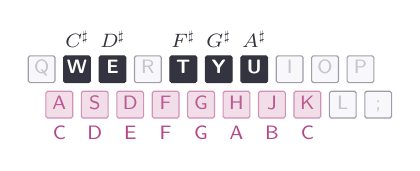
\begin{tikzpicture}
% Upper QWERTY row (sharps in DAW chromatic-staircase). Only 5 keys
% are mapped (W E T Y U); R and I sit in the gaps with no note.
\foreach \l/\note/\mapped [count=\i] in {%
 Q/{}/0, W/$C^\sharp$/1, E/$D^\sharp$/1, R/{}/0, T/$F^\sharp$/1,
 Y/$G^\sharp$/1, U/$A^\sharp$/1, I/{}/0, O/{}/0, P/{}/0%
}{
 \ifnum\mapped=1
  \node[kcap sharp] (k\i) at ({(\i-1)*0.45}, 1.8) {\strut\l};
  \node[font=\scriptsize\sffamily, text=keysharp, anchor=south, inner sep=1pt]
   at ({(\i-1)*0.45}, 2.03) {\note};
 \else
  \node[kcap, text=keystroke!60] (k\i) at ({(\i-1)*0.45}, 1.8) {\strut\l};
 \fi
}
% Home row (whites). 8 of 10 keys mapped (A through K = C..C).
\foreach \l/\note/\mapped [count=\i] in {%
 A/C/1, S/D/1, D/E/1, F/F/1, G/G/1, H/A/1, J/B/1, K/C/1, L/{}/0, {;}/{}/0%
}{
 \ifnum\mapped=1
  \node[kcap mapped] at ({(\i-1)*0.45+0.225}, 1.35) {\strut\l};
  \node[font=\scriptsize\sffamily, text=keymapped, anchor=north, inner sep=1pt]
   at ({(\i-1)*0.45+0.225}, 1.12) {\note};
 \else
  \node[kcap, text=keystroke!60] at ({(\i-1)*0.45+0.225}, 1.35) {\strut\l};
 \fi
}
\end{tikzpicture}}
\caption{El diseño AWSED --- el mapa de teclado cromático en escalera QWERTY-piano de los DAW (variante de Ableton, Logic, GarageBand). La fila de reposo \texttt{A~S~D~F~G~H~J~K} toca las teclas blancas de $C$ a $C$; la fila de arriba coloca los sostenidos en los huecos donde caerían las teclas negras del piano ($C^\sharp\,D^\sharp$ luego un hueco en \texttt{R}, $F^\sharp\,G^\sharp\,A^\sharp$, luego huecos). El nombre proviene de los primeros cinco tonos cromáticos $C\,C^\sharp\,D\,D^\sharp\,E$, que caen en \key{A}\,\key{W}\,\key{S}\,\key{E}\,\key{D}. La letra QWERTY de cada tecla no guarda relación con el nombre de la nota que produce.}
\label{fig:daw-staircase}
\end{figure}

Está también, argumentaré, mal diseñado. El diseño AWSED tiene tres debilidades estructurales. \textbf{Primera}, la letra QWERTY de cada tecla no guarda relación con el nombre de la nota que produce. \key{A} toca C; \key{S} toca D; \key{D} toca E (Figura~\ref{fig:daw-staircase}). Un usuario que haya aprendido la escala occidental de siete notas no obtiene ningún asidero sobre el mapa de teclado a partir de ese conocimiento. \textbf{Segunda}, entrega solo una única octava ($C$ a $C$), y sin embargo despliega esa única octava de extremo a extremo de la fila de reposo, de \key{A} a \key{K} --- todo el ancho donde descansan \emph{ambas} manos. No es ni una octava compacta para una mano ni un registro productivo para dos manos: gasta dos manos de teclado para producir una sola octava, y ahí se detiene. El ancho está dispuesto como para dos manos, pero el registro está dimensionado para una. \textbf{Tercera}, el mapa de teclado es ilegible sin un tutorial: no hay mnemotecnia, ni diagrama impreso en las teclas físicas, ni forma de derivar la asignación a partir de principios básicos. Un mapa de teclado que requiere un manual es un mapa de teclado que ha perdido su carácter de software social.

La denominación no fue ociosa. Su contraste natural es WASD, la convención de movimiento de los videojuegos de PC --- y el casi-anagrama no es una coincidencia sino más bien un diagnóstico. WASD tiene la misma forma estructural que AWSED --- una convención de entrada de usuario sin dueño, sin especificación y multiaplicación --- pero una historia de propagación distinta. Antes de WASD, los juegos de PC usaban por defecto las teclas de flecha (Wolfenstein 3D, Doom, la serie Quake hasta 1997)~\citep{wikipedia_arrow_keys}; entre los experimentos intermedios estuvieron el ASDX de System Shock (1994) y el AZ+QE de Descent. Dennis ``Thresh'' Fong, un jugador competitivo de Quake, popularizó el diseño WASD a través de su guía de configuración autopublicada~\citep{thresh_quake_bible} y ganó el primer torneo nacional de Quake en 1997. Half-Life de Valve distribuyó WASD por defecto en 1998, y para principios de los 2000 la convención había saturado los juegos de PC~\citep{fenlon2016wasd}. WASD persiste por una razón que la escalera cromática de los DAW no tiene: es genuinamente mejor que el valor por defecto oficial. Libera la mano derecha para el ratón, se sitúa contiguo a Shift / Space / Ctrl / Tab, y aprovecha la colocación de los dedos en la fila de reposo de un teclado QWERTY. La lección estructural es que la propagación es función de la mediación social \emph{y} de la aptitud: WASD se propagó porque la pedagogía de Fong llegó a los jugadores \emph{y} la asignación ganó por sus méritos. La escalera cromática se propagó solo a través de la pedagogía, a pesar de que los méritos corrían en sentido contrario. Ambos casos pertenecen a la misma categoría --- convenciones sin dueño que gobiernan la entrada del usuario a través de las aplicaciones. Demuestran que la categoría es lo bastante amplia como para abarcar tanto lo bien diseñado como lo mal diseñado, lo validado por el usuario y lo heredado por inercia.

\section{Notepat.com: notas que se nombran a sí mismas}
\label{sec:notepat}

Frente a este titular, \texttt{notepat.com} propone un mapa de teclado distinto (Figura~\ref{fig:notepat-keymap}). El principio de diseño es uno solo: \emph{notas que se nombran a sí mismas}. La letra QWERTY \key{C} toca C. La letra QWERTY \key{D} toca D. Las siete notas naturales de la escala occidental --- $C\,D\,E\,F\,G\,A\,B$ --- tocan las notas que sus letras nombran. La octava superior continúa alfabéticamente: \keys{H,I,J,K,L,M,N} para $C_5\,D_5\,E_5\,F_5\,G_5\,A_5\,B_5$. Los sostenidos se ubican una fila por encima de su nota natural, por analogía con las teclas negras de un piano, donde las letras QWERTY lo permiten: \keys{V,S,W,R,Q} para $C^\sharp\,D^\sharp\,F^\sharp\,G^\sharp\,A^\sharp$. La octava inferior cae bajo la mano izquierda; la octava superior cae bajo la derecha.

El mapa de teclado invierte cada una de las tres debilidades de AWSED. \textbf{Primera}, la letra de cada tecla \emph{es} el nombre de la nota. Cualquiera que conozca la escala occidental ya conoce el mapa de teclado. \textbf{Segunda}, gasta de forma productiva el ancho de las dos manos: la mano izquierda toca la octava inferior y la derecha la refleja en la superior, de modo que el mismo tramo que AWSED gasta en una única octava rinde dos. \textbf{Tercera}, el mapa de teclado se autodocumenta: el diagrama de la Figura~\ref{fig:notepat-keymap} puede reproducirse de memoria por cualquiera que sepa deletrear ``CDEFGAB''.

Tres cosas hacen que \texttt{notepat.com} sea inusual entre los mapas de teclado de este artículo: tiene nombre --- la mayoría, como AWSED (\textsection\ref{sec:daw}), nunca lo tuvieron --- sus notas se nombran a sí mismas, de modo que el mapa de teclado se dirige a sí mismo, y ya corre en muchas implementaciones. La contribución de \texttt{notepat.com} no es la implementación. La implementación es, por diseño, modesta: unos pocos cientos de líneas de JavaScript que enrutan eventos de teclado a una API de síntesis de audio. La contribución es el mapa de teclado. Se presenta en cinco implementaciones --- la pieza web en \texttt{notepat.com}, la adaptación a metal desnudo de AC Native OS, la aplicación de barra de menús de macOS MenuBand, el complemento de Ableton (Max for Live) y \texttt{babypat} --- y el mapa de teclado es lo único idéntico en todas ellas. La notación de denominación de notas viaja incluso más lejos que el instrumento: se reutiliza en \texttt{clock}, el secuenciador distribuido de AC, donde las mismas alturas de una sola letra impulsan la reproducción en red. Es el contrato de software social con forma de \texttt{notepat.com}.

Un lector que compare las implementaciones lado a lado notará teclas que hacen cosas más allá de la tabla de la Figura~\ref{fig:notepat-keymap}. En AC Native y MenuBand, mantener pulsado \texttt{Space} reproduce hacia atrás los últimos segundos de la salida de audio real. En la pieza web y AC Native, mantener \texttt{Shift} mientras se ataca una nota da a esa voz una larga cola de decaimiento al soltarla; mantener \texttt{Enter} sostiene la voz indefinidamente, y \texttt{Backspace} borra todas las voces sostenidas. En MenuBand y AC Native, \texttt{Control}, \texttt{Alt} y los dos juntos promueven una sola pulsación de tecla a una tríada mayor, menor o suspendida. Nada de esto aparece en el diagrama del mapa de teclado, y la omisión es deliberada. Estas combinaciones forman una \emph{capa de interpretación extendida}, y la línea entre esa capa y la asignación tonal es el límite del propio contrato de software social (Tabla~\ref{tab:contract-line}).

\begin{table}[t]
\footnotesize
\setlength{\tabcolsep}{3pt}
\renewcommand{\arraystretch}{1.05}
\centering
\caption{Las combinaciones de \texttt{notepat.com}, divididas en la línea del contrato. Por encima de la línea: la asignación tonal, idéntica en todas las implementaciones --- el objeto de software social. Por debajo: la capa de interpretación extendida, donde cada sustrato es libre de diferir.}
\label{tab:contract-line}
\begin{tabularx}{\columnwidth}{@{}>{\RaggedRight}p{0.30\columnwidth}>{\RaggedRight}X>{\RaggedRight\arraybackslash}p{0.21\columnwidth}@{}}
\toprule
\textbf{Combinación} & \textbf{Significado} & \textbf{Dónde} \\
\midrule
\multicolumn{3}{@{}l}{\emph{Contrato tonal}} \\[0.1em]
\texttt{C D E F G A B} & naturales $C_4$--$B_4$, mano izquierda & todas \\
\texttt{H I J K L M N} & naturales $C_5$--$B_5$, mano derecha & todas \\
\texttt{V S W R Q} & sostenidos, una fila arriba & todas \\
\midrule
\multicolumn{3}{@{}l}{\emph{Capa de interpretación extendida}} \\[0.1em]
\texttt{Shift} (mant.) & sostén: larga cola de decaimiento & web, Native \\
\texttt{Enter} (mant.) & sostiene la voz; \texttt{Backspace} borra & web, Native \\
\texttt{Space} (mant.) & reproduce hacia atrás el audio reciente & Native, MenuBand \\
\texttt{Ctrl}\,/\,\texttt{Alt}\,/\,ambos & tríada mayor\,/\,menor\,/\,sus2 & MenuBand, Native \\
\texttt{<}~\texttt{>} & cambio de octava por mano & web \\
\bottomrule
\end{tabularx}
\end{table}

Las dos mitades de la Tabla~\ref{tab:contract-line} se rigen por reglas distintas. Por encima de la línea, la desviación es ruptura: una implementación que reasignara \texttt{C} apartándola de la nota $C$ no sería una adaptación de \texttt{notepat.com} sino un instrumento distinto. Por debajo de la línea, la desviación es modismo: cada sustrato cultiva los gestos que su cuerpo permite. El SO de metal desnudo, dueño de toda la máquina, puede almacenar en un búfer circular su propia salida de audio y reproducirla al revés; la aplicación de barra de menús, montada sobre una captura de eventos de todo el sistema, se apoya en acordes de modificadores; la pieza web, que vive en una pestaña del navegador, sostiene y mantiene. Los usuarios no experimentan estas diferencias como ruptura, y ninguna implementación está obligada a llevar los gestos de otra. La misma estructura de dos niveles es visible en los casos más antiguos: el contrato QWERTY no dice nada sobre teclas de medios o capas \texttt{Fn}, que varían libremente según el fabricante sin que nadie llame a un ThinkPad una bifurcación de QWERTY; los movimientos centrales de Vim son contrato mientras que las combinaciones de los complementos son modismo. Un mapa de teclado, esto sugiere, no es el conjunto de todas las combinaciones que distribuye una implementación. Es el subconjunto cuya alteración la comunidad experimentaría como una vulneración de la identidad --- y una prueba práctica de a qué lado de la línea cae una combinación es si la superficie de notación (\textsection\ref{sec:notation}) la lleva. \texttt{C D E F G A B} viaja como texto; ``mantén el espacio para invertir el tiempo'' es un gesto por sustrato que debe reenseñarse, mediante demostración, en cada adaptación.

Este es el movimiento que el artículo pide al lector que vea. El mapa de teclado dominante de escalera cromática de los DAW nunca fue \emph{elegido} --- fue \emph{heredado} del software de tracker, sostenido por la expectativa del usuario y enclaustrado por la convención multiaplicación. \texttt{notepat.com} demuestra que la brecha está abierta: que una alternativa diseñada deliberadamente puede ser autorizada por un único desarrollador en unos pocos cientos de líneas de código, distribuida en múltiples implementaciones en un año, y ofrecida a una comunidad más amplia como un contrato de software social rival. La apuesta política es pequeña en cualquier instancia aislada y grande en conjunto: \emph{la brecha está abierta en todas partes}.

\section{Notación: la superficie discursiva}
\label{sec:notation}

El argumento hasta aquí ha tratado el mapa de teclado como una tabla. Pero un mapa de teclado no es solo una tabla. También tiene una \emph{notación} --- una forma textual en la que el uso del mapa de teclado se lee, escribe, enseña, cita y discute. La notación es la superficie discursiva del mapa de teclado. Es también, argumentaré, la mitad del mapa de teclado que realmente viaja. Un mapa de teclado cuya notación es portátil se propaga como texto; un mapa de teclado cuya notación es torpe o ausente se propaga solo como memoria muscular. La calidad de la notación es por tanto una propiedad diseñable del mapa de teclado, no un artefacto derivado. Un diseñador que distribuye solo la tabla de combinaciones ha distribuido la mitad del objeto.

El caso canónico es Vim. El mapa de teclado subyacente de Vim es una tabla que asigna pulsaciones a comandos del editor: \texttt{d} inicia un operador de borrado, \texttt{i} un objeto de texto interno, \texttt{w} un movimiento de palabra. Lo que viaja en el discurso de Vim, sin embargo, no es la tabla. Lo que viaja es una \emph{notación}: \texttt{dd}, \texttt{ciw}, \texttt{gg}, \texttt{:wq}, \texttt{<C-w>} (Figura~\ref{fig:vim-modes}). Los tutoriales, las entradas de blog, los archivos README, vimtutor y la duradera discusión vim-contra-emacs se conducen todos en esta notación. La notación es tan portátil que sobrevive por completo fuera de Vim: el \emph{modo vim} aparece en Visual Studio Code, en JupyterLab, en las shells mediante \texttt{set -o vi}, en los campos de texto Cocoa de macOS, en los navegadores mediante Vimium. Lo que se está portando es la notación. El entorno de ejecución es contingente.

\begin{figure}[t]
\centering
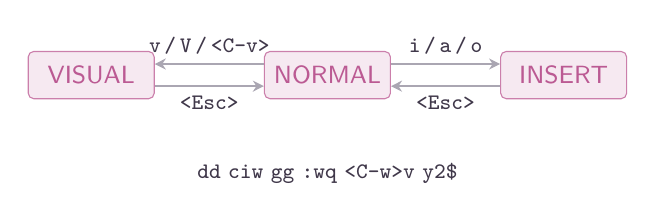
\begin{tikzpicture}[
 modebox/.style={draw=keymapped!70, fill=keymapped!12,
          rounded corners=2pt, minimum width=1.6cm,
          minimum height=0.6cm, font=\small\sffamily,
          text=keymapped!90, inner sep=2pt},
 arrow/.style={-{Stealth[length=4pt,width=4pt]}, draw=keystroke!90,
         line width=0.5pt},
 cmd/.style={font=\footnotesize\ttfamily, text=acdark}
]
% Three Vim modes wired by their command-notation transitions.
\node[modebox] (normal) at (0, 0) {NORMAL};
\node[modebox] (insert) at (3.0, 0) {INSERT};
\node[modebox] (visual) at (-3.0, 0) {VISUAL};
\draw[arrow] ([yshift=4pt]normal.east) -- node[above, cmd] {\texttt{i}\,/\,\texttt{a}\,/\,\texttt{o}} ([yshift=4pt]insert.west);
\draw[arrow] ([yshift=-4pt]insert.west) -- node[below, cmd] {\texttt{<Esc>}} ([yshift=-4pt]normal.east);
\draw[arrow] ([yshift=4pt]normal.west) -- node[above, cmd] {\texttt{v}\,/\,\texttt{V}\,/\,\texttt{<C-v>}} ([yshift=4pt]visual.east);
\draw[arrow] ([yshift=-4pt]visual.east) -- node[below, cmd] {\texttt{<Esc>}} ([yshift=-4pt]normal.west);
% A row of canonical commands underneath
\node[font=\footnotesize\ttfamily, text=acdark, anchor=north] at (0, -1.0)
 {\texttt{dd}\,\,\texttt{ciw}\,\,\texttt{gg}\,\,\texttt{:wq}\,\,\texttt{<C-w>v}\,\,\texttt{y2}\$};
\end{tikzpicture}
\caption{El mapa de teclado modal de Vim y su notación viajera. Los modos (NORMAL, INSERT, VISUAL) están conectados por transiciones de pulsaciones etiquetadas; los comandos comunes (\texttt{dd} borrar-línea, \texttt{ciw} cambiar-palabra-interna, \texttt{gg} ir-arriba, \texttt{:wq} escribir-y-salir, etc.) son la moneda discursiva del mapa de teclado. La notación es tan portátil que se ha reimplementado en VS~Code, JupyterLab, Vimium, el sistema de texto Cocoa de macOS y \texttt{set -o vi}.}
\label{fig:vim-modes}
\end{figure}

La escalera cromática de los DAW es el caso negativo. No hay notación portátil para ella. Escribir una melodía tocada con el tecleo musical de Ableton exige recurrir a una prosa de secuencia de eventos --- ``pulsa \key{A}, luego \key{S}, luego \key{D}'' --- que describe la entrada en vez de la música. Compárese con la notación de cubo de Singmaster~\citep{singmaster1981notes} (Figura~\ref{fig:singmaster}), donde \texttt{R U R' U' R U2 R'} permite que un algoritmo del cubo de Rubik viaje intacto entre cuberos; o con el Nashville Number System~\citep{matthews1984nashville,williams1988nashville}, donde ``1--4--5'' permite que una progresión de acordes viaje entre músicos de sesión; o con la teoría estenográfica de Plover~\citep{knight2010plover}, donde la notación de acordes permite que los patrones estenográficos viajen a través de un diccionario editado por la comunidad. La escalera de los DAW no tiene tal asidero. Sus teclas solo son direccionables por su posición física. El mapa de teclado existe por tanto en la memoria muscular y rara vez sobre el papel --- que es exactamente por lo que tiene menor presencia discursiva que Vim a pesar de una base de usuarios posiblemente mayor.

\begin{figure}[t]
\centering
\resizebox{0.62\columnwidth}{!}{%
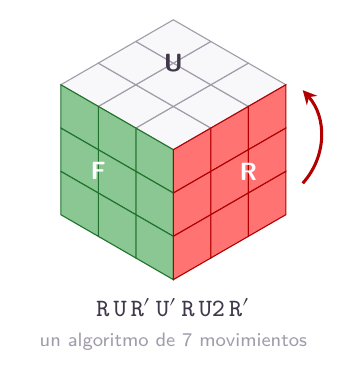
\begin{tikzpicture}
% Symmetric bounding box around the cube body (x=0) so \centering
% lands it centered --- the quarter-turn arrow otherwise extends the
% natural box rightward and pulls the cube off-center.
\useasboundingbox (-1.85,-2.55) rectangle (1.85,1.55);
% Isometric Rubik's cube, three visible faces: U (top), F (front-
% left), R (right). Faces are explicit-path parallelogram grids built
% from iso axes er=(0.866,0.5)s (right-up), el=(-0.866,0.5)s
% (left-up), ed=(0,-1)s (down), all meeting at the shared front-top
% vertex at the origin. The R face is tinted with a quarter-turn
% arrow: the diagram shows the first move of the algorithm below.
\def\s{0.55}
% Top face U: cells spanned by er and el
\foreach \i in {0,1,2} \foreach \j in {0,1,2}
 \draw[keystroke, fill=keyfill]
  ({0.866*\s*(\i-\j)}, {0.5*\s*(\i+\j)})
  -- ++({0.866*\s}, {0.5*\s})
  -- ++({-0.866*\s}, {0.5*\s})
  -- ++({-0.866*\s}, {-0.5*\s}) -- cycle;
% Front-left face F: cells spanned by el and ed — green stickers
\foreach \i in {0,1,2} \foreach \j in {0,1,2}
 \draw[acgreen!75!black, fill=acgreen!55]
  ({-0.866*\s*\i}, {0.5*\s*\i - \s*\j})
  -- ++({-0.866*\s}, {0.5*\s})
  -- ++(0, {-\s})
  -- ++({0.866*\s}, {-0.5*\s}) -- cycle;
% Right face R: cells spanned by er and ed — red stickers (mid-turn)
\foreach \i in {0,1,2} \foreach \j in {0,1,2}
 \draw[red!70!black, fill=red!55]
  ({0.866*\s*\i}, {0.5*\s*\i - \s*\j})
  -- ++({0.866*\s}, {0.5*\s})
  -- ++(0, {-\s})
  -- ++({-0.866*\s}, {-0.5*\s}) -- cycle;
% Face labels at face centers — standard sticker scheme:
% white up, green front, red right.
\node[font=\small\sffamily\bfseries, text=acdark]
 at (0, {1.5*\s + 0.5*\s}) {U};
\node[font=\small\sffamily\bfseries, text=white]
 at ({-0.866*\s*1.5 - 0.433*\s}, {0.75*\s - 1.5*\s + 0.25*\s}) {F};
\node[font=\small\sffamily\bfseries, text=white]
 at ({0.866*\s*1.5 + 0.433*\s}, {0.75*\s - 1.5*\s + 0.25*\s}) {R};
% Quarter-turn arrow for R: curved arrow hugging the right face's
% outer edge, pointing upward (clockwise as seen from the right).
\draw[-{Stealth[length=5pt,width=5pt]}, line width=1.1pt, red!70!black]
 ({0.866*\s*3.45}, {0.5*\s*3.45 - 2.5*\s})
 to[bend right=42]
 ({0.866*\s*3.45}, {0.5*\s*3.45 - 0.35*\s});
% Notation row underneath
\node[font=\small\ttfamily, anchor=north, text=acdark]
 at (0, {-3.2*\s}) {R\,U\,R$'$\,U$'$\,R\,U2\,R$'$};
\node[font=\scriptsize\sffamily, anchor=north, text=keystroke]
 at (0, {-4.0*\s}) {un algoritmo de 7 movimientos};
\end{tikzpicture}}
\caption{La notación de cubo de Singmaster~\citep{singmaster1981notes}. Cada letra mayúscula nombra una cara (\textsf{U}p/arriba, \textsf{D}own/abajo, \textsf{L}eft/izquierda, \textsf{R}ight/derecha, \textsf{F}ront/frente, \textsf{B}ack/atrás); una letra sola es un cuarto de giro horario, una letra con prima ($\,'$) un cuarto de giro antihorario, y un dígito 2 un medio giro. La cadena de siete símbolos \texttt{R U R$'$ U$'$ R U2 R$'$} es un algoritmo completo portátil entre cuberos, repositorios de GitHub y tutoriales de YouTube --- el par mapa de teclado-notación viajando como texto. Las caras llevan el esquema de pegatinas estándar (blanco arriba, verde al frente, rojo a la derecha); \textsf{R} está dibujada a medio cuarto de giro: el primer movimiento del algoritmo.}
\label{fig:singmaster}
\end{figure}

El diseño ``las notas se nombran a sí mismas'' de \texttt{notepat.com} tiene, como efecto secundario estructural, una notación que no cuesta nada aprender. Para escribir una secuencia de notepat.com, se escribe \texttt{C D E F G A B} --- que es también notación musical estándar. La notación no se inventa para \texttt{notepat.com}; se \emph{hereda} de una alfabetización existente. Un pianista que nunca ha visto un mapa de teclado de notepat.com puede leer una partitura de notepat.com; a la inversa, un intérprete de notepat.com que aprende el mapa de teclado está también ensayando la alfabetización estándar de letras-altura. Así se ve una superficie de notación bien diseñada: la notación es tan trivialmente derivable del conocimiento previo que aprenderla no cuesta nada. La escalera cromática de Ableton, en cambio, exigiría que una partitura al estilo de notepat se recodificara como \texttt{A S D F G H J} --- una notación privada atada a un solo mapa de teclado, inútil en ningún otro lugar.

La literatura empírica sobre la adopción de atajos de teclado respalda esta lectura. Peres et al.\ hallaron que trabajar junto a otros usuarios de atajos predice el uso de atajos con más fuerza que la experiencia informática por sí sola~\citep{peres2004shortcut}. Lozhkina et al.\ extienden el resultado: el canal de descubrimiento de los atajos es interpersonal y visual~\citep{lozhkina2025discovery}. Wang et al.\ usan explícitamente el término \emph{vocabulario} para nombrar lo que el diseño de atajos entrega a un usuario~\citep{wang2020keymap}. El argumento de este artículo afina esos hallazgos: la mediación social no es un efecto genérico de estar-rodeado-de-otros-usuarios; es una transmisión específica a través de la superficie de notación. Los colegas leen las pantallas de los demás, ven \texttt{:wq}, preguntan, aprenden. Donde no hay notación transmisible, no hay mediación social que mediar. La misma lógica explica el éxito de las mini-notaciones de codificación en vivo: el lenguaje de patrones TidalCycles de Alex McLean y Geraint Wiggins~\citep{mclean2010tidal}, portado a JavaScript como Strudel~\citep{roos2023strudel}, y las cadenas de transformación de Hydra de Olivia Jack para visuales codificados en vivo~\citep{jack2018hydra}, junto a la notación ABC para la música folk~\citep{walshaw_abc}. En cada caso el entorno de ejecución es contingente --- Haskell, JavaScript, WebGL, reproductores MIDI --- pero la notación lleva la práctica a través de entornos de ejecución, talleres y décadas.

El catálogo de corolarios de \textsection\ref{sec:corollaries} es, leído a través de esta lente, casi por entero un catálogo de notaciones. Singmaster, Nashville, ABC, AFI, Camelot, la notación de pad numérico de los juegos de lucha, la altura científica, el alfabeto de deletreo de la OTAN, las abreviaturas de tejido --- cada una es una notación derivada de un mapa de teclado (o asignación de entrada) que permitió que la práctica subyacente viajara como texto. El par mapa de teclado-notación es la unidad. El mapa de teclado aporta la posibilidad; la notación aporta la superficie de propagación.

La afirmación estructural tiene un diagnóstico más profundo. La distinción de Walter Ong entre oralidad y escritura~\citep{ong1982orality}, construida sobre el relato de Havelock de esa misma transición en la antigua Grecia~\citep{havelock1963preface}, corta la cuestión con limpieza. Las tradiciones \emph{orales} persisten mediante la interpretación, la transmisión de persona a persona y la aproximación repetida; no tienen texto canónico, mutan ligeramente entre instancias y sobreviven porque los intérpretes siguen interpretándolas. Las tradiciones \emph{escritas} persisten mediante texto fijo, ediciones autorizadas y reproducción exacta; tienen especificaciones, cánones e implementaciones de referencia. Los marcos habituales de la academia informática son todos marcos escritos: una licencia de código abierto gobierna un texto fijo, un protocolo gobierna un formato de cable fijo, un formato gobierna una codificación fija. La escalera cromática de los DAW es un mapa de teclado de oralidad primaria --- no hay texto canónico, solo cuatro implementaciones que coinciden por interpretación. Vim tiene a la vez un sustrato oral (uno aprende el mapa de teclado mirando la pantalla de otro desarrollador) y un filo escrito (la notación: \texttt{:wq}, \texttt{<C-w>}, \texttt{ciw}). \texttt{notepat.com} colapsa el lado escrito en la alfabetización vigente de la notación de letras-altura: el mapa de teclado hereda su forma escrita de una práctica escrita siglos más antigua. El sustrato oral es el mapa de teclado; la notación es la fijación escrita; donde esta última triunfa, el primero gana un cuerpo que viaja. El eje oralidad-escritura es el diagnóstico de por qué los mapas de teclado escapan del marco código abierto/propietario en absoluto: los marcos habituales son marcos escritos, pero el mapa de teclado es al menos en parte oral, y la ausencia de una fijación escrita tanto en el discurso académico como en el industrial es el síntoma que dio a este artículo su pregunta motivadora.

El mismo eje oralidad-escritura explica un rasgo de la literatura sobre mapas de teclado: casi no la hay. La historia de WASD de PC Gamer~\citep{fenlon2016wasd} es la fuente canónica de prensa popular sobre una convención que controla cientos de millones de horas de juego; la literatura académica equivalente está esencialmente vacía. Eso no es porque los mapas de teclado carezcan de importancia. Es porque el aparato existente de la academia informática --- especificaciones, RFC, repositorios de código fuente --- está calibrado para artefactos escritos, y un mapa de teclado es en parte oral. El artículo que no existe es exactamente el que este artículo sostiene que debería existir.

\section{El catálogo de corolarios}
\label{sec:corollaries}

El mapa de teclado es una instancia de un género mucho mayor: \emph{objetos virtuales versionados que se propagan mediante contrato social, no mediante binarios}. La Tabla~\ref{tab:corollaries} cataloga las principales especies. El catálogo no es exhaustivo. Su propósito es mostrar que el género es real y grande.


Emergen varios patrones. Primero, el género abarca asignaciones de entrada (QWERTY, Vim, WASD), sistemas notacionales (Singmaster, Nashville, AFI), etiquetas de categoría (botones de mando, colores CSS) e iniciales autorizadas por comunidades (el alfabeto de deletreo de la OTAN; el acrónimo LGBTQ+, cuyo historial de revisiones --- LGB $\rightarrow$ LGBT $\rightarrow$ LGBTQ $\rightarrow$ LGBTQIA $\rightarrow$ LGBTQIA2S+ --- es en sí mismo un proceso versionado-sin-órgano-rector documentado en guías de estilo~\citep{glaad_reference_guide}). Lo que los unifica no es el medio sino el \emph{papel}: cada uno es una pequeña tabla declarativa consultada en un límite entre humano y máquina, entre comunidades de práctica, o entre implementaciones rivales. Segundo, el patrón del inventor nombrado es muy variable. Algunos objetos tienen un único inventor nombrado (Singmaster, Coleman, Davis); otros tienen orígenes convergentes o anónimos (escalera cromática de los DAW, notación de pad numérico de los juegos de lucha); otros están versionados por la comunidad con añadidos nombrados (las iniciales LGBTQ+); otros se cristalizan por federación tras un período de competencia comunitaria (ajedrez algebraico, BÉPO). Tercero, el mecanismo de propagación casi nunca es un binario. Es la pedagogía, la expectativa, la cita o la referencia escrita --- el aparato de una comunidad escrita.

Vale la pena trazar con nitidez el límite de la categoría. Los \textbf{formatos abiertos} como PNG y MP3 se rigen por especificaciones e implementaciones de referencia~\citep{sterne2012mp3} --- más cerca del formato que del software social. Los \textbf{protocolos abiertos} como HTTP e IRC tienen RFC y órganos administradores --- \emph{Protocol} de Galloway~\citep{galloway2004protocol} cubre ese terreno. Las \textbf{folksonomías} (etiquetas, hashtags) son clasificación de contenido más que interfaz-como-objeto. Los \textbf{memes} se propagan pero son contenido. El mapa de teclado es distinto de todos estos: \emph{una pequeña tabla declarativa que media la entrada/salida, sin órgano rector, que sin embargo se comporta como si estuviera estandarizada}.

% X cells render as m{} (vertically centered, footnotesize) so single
% -line labels sit centered against wrapped propagation text. Defined
% OUT here (not inside \afterpage — a bare #1 breaks its tokenizer).
\renewcommand{\tabularxcolumn}[1]{>{\footnotesize}m{#1}}
% Full-width table as a proper float page ([p]): LaTeX fills the
% surrounding two-column text pages completely (no stranded column)
% and drops the table on its own float page. Label columns auto-size
% and never wrap; only the Propagation column flexes.
\begin{table*}[p]
\footnotesize
\setlength{\tabcolsep}{5pt}
\renewcommand{\arraystretch}{1.32}
\centering
\caption{Objetos virtuales versionados seleccionados que se propagan mediante contrato social. ``Originador'' lista al inventor nombrado cuando existe uno; ``\emph{conv.}'' indica un origen convergente o anónimo. El código QR de cada fila resuelve al hogar canónico del objeto --- Wikipedia, el sitio propio del proyecto o su especificación rectora.}
\label{tab:corollaries}
\arrayrulecolor{acgray!35}
\begin{tabularx}{\textwidth}{|@{\hspace{2.5pt}}c@{\hspace{2.5pt}}|>{\bfseries\color{acdark}}l|>{\color{acdark}}l|l|>{\RaggedRight\arraybackslash\color{acdark}}X|}
\hline
\cellcolor{acdark!75}{\color{white}\bfseries Escanear} &
\cellcolor{acpink!75}{\color{white}\bfseries Objeto} &
\cellcolor{acpurple!75}{\color{white}\bfseries Originador (año)} &
\cellcolor{acblue!75}{\color{white}\bfseries Dominio} &
\cellcolor{acgreen!75}{\color{white}\bfseries Propagación} \\
\hline
\rowcolor{acblue!8} \qrc{qwerty} & QWERTY            & Sholes (1873)               & \dmn{acblue}{Escritura}  & Adopción de fabricantes $\rightarrow$ ISO/AFNOR $\rightarrow$ archivos de diseño del SO \\ \hline
\rowcolor{acblue!8} \qrc{dvorak} & Dvorak            & Dvorak \& Dealey (1936)          & \dmn{acblue}{Escritura}  & Patente de EE.\,UU.\ $\rightarrow$ Marina de EE.\,UU.\ $\rightarrow$ diseños del SO instalados por el usuario \\ \hline
\rowcolor{acblue!8} \qrc{colemak} & Colemak           & Coleman (2006)               & \dmn{acblue}{Escritura}  & colemak.com + bifurcaciones de GitHub (Workman, Halmak, DH) \\ \hline
\rowcolor{acblue!8} \qrc{bepo} & BÉPO             & Comunidad (2005)              & \dmn{acblue}{Escritura}  & Diseño comunitario $\rightarrow$ norma estatal AFNOR de 2019 \\ \hline
\rowcolor{acpink!8} \qrc{janko} & Janko            & Jankó (1882)                & \dmn{acpink}{Música}   & \emph{Propagación fallida} --- estudio de caso negativo \\ \hline
\rowcolor{acpink!8} \qrc{wicki} & Wicki--Hayden         & Wicki (1896) / Hayden (1986)        & \dmn{acpink}{Música}   & Comunidad de concertina $\rightarrow$ controladores MPE modernos \\ \hline
\rowcolor{acpink!8} \qrc{bosanquet} & Bosanquet          & Bosanquet (1875)              & \dmn{acpink}{Música}   & Comunidad microtonal $\rightarrow$ Lumatone \\ \hline
\rowcolor{acpink!8} \qrc{daw} & AWSED (escalera de DAW) & \emph{conv.} (trackers, años 90)       & \dmn{acpink}{Música}   & Pedagogía entre DAW; expectativa del usuario \\ \hline
\rowcolor{acgreen!8} \qrc{wasd} & Movimiento WASD        & Fong (1996--97)              & \dmn{acgreen}{Juegos}  & Pedagogía de Quake $\rightarrow$ Half-Life por defecto $\rightarrow$ norma de la industria~\citep{fenlon2016wasd,thresh_quake_bible} \\ \hline
\rowcolor{acpink!8} \qrc{notepat} & Notepat ``se nombran solas'' & Scudder (2024)               & \dmn{acpink}{Música}   & Contrato entre implementaciones dentro de \ac{} \\ \hline
\rowcolor{acblue!8} \qrc{plover} & Teoría estenográfica Plover     & Knight (años 2010)               & \dmn{acblue}{Escritura}  & GitHub + diccionarios bifurcados por la comunidad \\ \hline
\rowcolor{acpurple!8} \qrc{vim} & Combinaciones de Vim       & Joy (1976) $\rightarrow$ Moolenaar (1991) & \dmn{acpurple}{Edición} & ``Combinaciones de Vim en todas partes''; campos de texto Cocoa de macOS \\ \hline
\rowcolor{acorange!8} \qrc{singmaster} & Notación Singmaster     & Singmaster (1981)             & \dmn{acorange}{Rompecabezas} & Folleto de Penguin $\rightarrow$ adopción universal entre cuberos \\ \hline
\rowcolor{acorange!8} \qrc{chess} & Notación algebraica de ajedrez   & Stamma (1737) $\rightarrow$ FIDE (1981)  & \dmn{acorange}{Juego}  & Cristalización federativa de convenciones comunitarias \\ \hline
\rowcolor{acpink!8} \qrc{nashville} & Nashville Number System   & Matthews (1957) / Williams (1988)     & \dmn{acpink}{Música}   & Tradición oral de músicos de sesión + libro autopublicado \\ \hline
\rowcolor{acpink!8} \qrc{abc} & Notación ABC         & Walshaw (años 80)              & \dmn{acpink}{Música}   & Intercambio de melodías folk en texto plano por listas de correo \\ \hline
\rowcolor{acpink!8} \qrc{helmholtz} & Altura Helmholtz / científica & Helmholtz (1863) / Sauveur (1713)     & \dmn{acpink}{Música}   & Manuales de acústica + documentación MIDI \\ \hline
\rowcolor{acpink!8} \qrc{camelot} & Rueda Camelot        & Davis (1991)                & \dmn{acpink}{DJing}   & Mixed In Key + toda herramienta de detección de tonalidad \\ \hline
\rowcolor{acgreen!8} \qrc{numpad} & Notación de pad numérico (236P)    & \emph{conv.} (FGC japonesa)        & \dmn{acgreen}{Juegos}  & Wikis, subreddits de emparejamiento \\ \hline
\rowcolor{acpink!8} \qrc{tidal} & Mini-notación TidalCycles  & McLean \& Wiggins (2010)          & \dmn{acpink}{Música}   & Tidal Club + talleres + patrones de GitHub~\citep{mclean2010tidal} \\ \hline
\rowcolor{acpink!8} \qrc{strudel} & Mini-notación Strudel    & Roos \& McLean (2023)           & \dmn{acpink}{Música}   & Editor de navegador + pedagogía ICLC~\citep{roos2023strudel} \\ \hline
\rowcolor{acpink!8} \qrc{hydra} & Cadenas de transformación Hydra    & Jack (2018)                & \dmn{acpink}{Visuales}  & Navegador + gists compartidos~\citep{jack2018hydra} \\ \hline
\rowcolor{acgray!12} \qrc{ipa} & AFI             & Asociación del AFI (1888)           & \dmn{acgray}{Fonética} & Estandarizado por federación; revisado en Kiel 1989 \\ \hline
\rowcolor{acgray!12} \qrc{nato} & Alfabeto de deletreo OTAN    & ICAO (1956)                & \dmn{acgray}{Aviación} & Estandarizado por federación \\ \hline
\rowcolor{acgray!12} \qrc{lgbtq} & Iniciales LGBTQ+      & Comunidad (años 80--)            & \dmn{acgray}{Identidad} & Guías de estilo (GLAAD); revisado mediante el uso~\citep{glaad_reference_guide} \\ \hline
\rowcolor{acgreen!8} \qrc{controller} & Botones de mando      & Nintendo (1990) / Goto (1994)       & \dmn{acgreen}{Juegos}  & Las versiones distribuyen ambos juegos de etiquetas (A/B/X/Y \emph{frente a}\ $\triangle\,\bigcirc\,\times\,\mdlgwhtsquare$) \\ \hline
\rowcolor{acgray!12} \qrc{css} & Colores con nombre de CSS       & X11 (1987) $\rightarrow$ SVG (2001)    & \dmn{acgray}{Web}    & Heredado sin cambios entre navegadores \\ \hline
\rowcolor{acgray!12} \qrc{knitting} & Abreviaturas de tejido    & Craft Yarn Council / RU          & \dmn{acgray}{Artesanía}   & Impresas en todo patrón \\ \hline
\end{tabularx}
\arrayrulecolor{black}
\end{table*}

\section{Leyendo a través de Lialina}
\label{sec:lialina}

El ensayo \emph{Turing Complete User} de Olia Lialina~\citep{lialina2012turing,lialina2021turingbook} es el ancla teórica portante de este artículo. Lialina sostiene que la categoría ``usuario'' está siendo silenciosamente eliminada del diseño de software contemporáneo, reemplazada por un registro que se dirige a las personas sin reconocer la agencia que las hizo usuarios en primer lugar. El argumento es moral y político: ``Necesitamos cuidar de esta palabra porque dirigirse a personas y no a usuarios oculta la existencia de dos clases de personas --- desarrolladores y usuarios''~\citep{lialina2012turing}. Su tesis es que los usuarios son programadores en espera; el sustrato debe seguir siendo programable para que la agencia sea real.

El mapa de teclado, argumento, es exactamente la superficie donde el argumento de Lialina encuentra expresión material. Lialina nombra la condición que hace posible la autoría del usuario: ``una situación en la que el flujo de trabajo de una aplicación tiene brechas que pueden ser rellenadas por los usuarios, donde la suavidad y la ausencia de costuras se rompen''~\citep{lialina2012turing}. El mapa de teclado es una de esas brechas. El hardware es fijo; el binario es cerrado; pero la tabla que asigna la tecla QWERTY \key{A} al MIDI 60 puede ser autorizada por el usuario, versionada por el usuario y reclamada por el usuario entre aplicaciones. Cuando las aplicaciones cierran esa brecha --- fijan una asignación, rechazan alternativas, ocultan la tabla tras una capa de UX que no admite ediciones --- el usuario-como-autor muere en esa superficie. Esto es lo que Lialina, en su ensayo complementario~\citep{lialina2018rich}, llama \emph{desktopización}: la colonización de las superficies configurables por el usuario por parte de una UX gestionada. El mapa de teclado es el canario.

El catálogo de corolarios de \textsection\ref{sec:corollaries} afina el punto. Cada entrada de la Tabla~\ref{tab:corollaries} es una superficie sobre la que una comunidad de usuarios ha autorizado una pequeña tabla declarativa que la tecnología subyacente no requería. La escala occidental no requiere la notación ABC; el teclado QWERTY no requiere la teoría estenográfica de Plover; el cubo de Rubik no requiere la notación de Singmaster; la escala cromática en temperamento igual de 12 tonos no requiere el mapa de teclado ``se nombran solas'' de notepat.com. Cada una es una pieza de convención autorizada por el usuario que sobrevive y se propaga porque una comunidad decidió que así debía ser.

La apuesta política de \emph{Turing Complete User} es la preservación de estas superficies. La contribución de este artículo es dar a las superficies un nombre --- \emph{software social} --- y demostrar, por enumeración, que la categoría es lo bastante grande como para ser políticamente consecuente. El argumento de \textsection\ref{sec:notation} afina la afirmación política: donde el mapa de teclado tiene una notación portátil, la autoría del usuario es legible para otros usuarios; donde no la tiene, el mapa de teclado muere en la memoria muscular y el contrato de software social se vuelve invisible incluso para las personas que lo sostienen. La desaparición de cualquier mapa de teclado aislado es pequeña. La desaparición de toda la capa que el usuario puede autorizar es la desaparición del usuario de Lialina. La desaparición de la \emph{superficie de notación} es la desaparición de la voz del usuario, además de la mano del usuario.

\section{Lo que esto exige a los diseñadores}
\label{sec:design}

Si el argumento de \textsection\ref{sec:lialina} es correcto --- si los mapas de teclado son el cuerpo empírico del Turing Complete User --- entonces se sigue una petición pequeña y concreta para los diseñadores de cualquier sistema que consuma un mapa de teclado. \textbf{Distribuya el mapa de teclado como un objeto de primera clase.} Hágalo legible: imprima la tabla en algún lugar donde un usuario pueda verla. Hágalo exportable: permita que un usuario guarde la tabla en un archivo. Hágalo bifurcable: permita que un usuario cargue una tabla distinta. Documente el formato: prefiera una tabla en texto plano a un binario opaco. Prefiera una convención publicada a una privada. Prefiera un mapa de teclado compartido por la comunidad a uno exclusivo del fabricante.

\textbf{Y distribuya la notación también como un objeto de primera clase} (\textsection\ref{sec:notation}). El mapa de teclado es la mitad del artefacto; la notación es la otra mitad. Un mapa de teclado cuya notación es torpe, intranscribible o inventada desde cero quedará latente en la memoria muscular. Un mapa de teclado cuya notación es escueta, tipográfica y derivable de la alfabetización comunitaria existente viajará como texto, se propagará a través de tutoriales y sobrevivirá a su entorno de ejecución actual. Las dos preguntas de diseño son inseparables: cuando eliges una combinación, eliges también cómo se escribirá, enseñará y portará esa combinación.

\texttt{notepat.com} distribuye su mapa de teclado como la Figura~\ref{fig:notepat-keymap} --- un diagrama de una página, libremente reproducible, presente en cada implementación. La escalera cromática de los DAW distribuye su mapa de teclado como un tutorial enterrado en un manual, idéntico entre aplicaciones por accidente, propiedad de nadie e impugnable por nadie. La diferencia no es técnica. La diferencia es si el contrato de software social se trata como un objeto explícito o uno implícito.

\section{Conclusión}

Un mapa de teclado es una pequeña tabla declarativa. No es un binario. No es un servicio. No es un proyecto. Los marcos habituales de la academia informática no logran verlo. Y sin embargo los mapas de teclado están versionados, nombrados, bifurcados y reclamados entre aplicaciones --- son software en todo sentido que importa. He argumentado que constituyen una categoría, he llamado a la categoría \emph{software social}, he rastreado dos linajes que la produjeron, he examinado el caso contemporáneo dominante (la escalera cromática de los DAW) y una intervención deliberada contra él (las notas-que-se-nombran-a-sí-mismas de \texttt{notepat.com}), he mostrado que cada mapa de teclado tiene una \emph{superficie de notación} que es a menudo la mitad del artefacto que realmente viaja, he enumerado un catálogo más amplio de corolarios que son ellos mismos predominantemente notaciones, y he leído el cuerpo de pruebas a través del \emph{Turing Complete User} de Lialina como apoyo a su afirmación de que los usuarios son programadores en espera. La desaparición de cualquier mapa de teclado individual es pequeña. La desaparición de toda la capa que el usuario puede autorizar es el problema político que Lialina nombra.

La contribución metodológica es una unidad de análisis: el mapa de teclado-y-su-notación como el objeto de primera clase de la academia informática que el binario, el proyecto, la plataforma y el formato juntos no logran resolver. Leído a través de Ong, el mapa de teclado es el artefacto en parte oral y la notación es su filo escrito --- razón por la que ni el mapa de teclado solo ni la notación sola bastan, y por la que los marcos habituales de la academia informática, calibrados como están para artefactos plenamente escritos, pasan por alto la categoría por completo. La contribución política es una petición pequeña: \emph{distribuya el mapa de teclado como un objeto de primera clase, y la notación junto a él}.

\section*{Agradecimientos}

Este artículo se escribió durante la residencia del autor en \emph{Social Software}, la iniciativa de UCLA Design\,\textbar\,Media Arts dirigida por Lauren Lee McCarthy y Casey Reas~\citep{sosoft_info}, como parte de su segundo ciclo, \emph{Scores for Social Software}, dirigido por Casey Reas, de abril a junio de 2026~\citep{reas2026scores}. El planteamiento del ciclo de la partitura como una forma de coreografiar acontecimientos en el tiempo mediante texto, diagramas y otras formas de instrucción dio forma al argumento sobre la notación de \textsection\ref{sec:notation}, y la definición de software social de la iniciativa --- cualquier sistema que organiza el comportamiento, coordina a las personas o estructura la interacción --- es el contexto de trabajo para la categoría que este artículo nombra. Gracias a la cohorte por diez semanas de partituras.\hspace{3pt}\raisebox{-5pt}{\rotatebox{-12}{
\includegraphics[height=26pt]{figures/pals-pink.png}}}

\appendix
\renewcommand{\thesection}{Apéndice~\Alph{section}}

\section{El mapa de teclado y el módulo: Notepat después de John Holden}
\label{app:holden}

En 1770 un alfarero de Glasgow llamado John Holden publicó un \emph{Essay towards a Rational System of Music} que, como ha mostrado Carmel Raz, se anticipó a la ciencia cognitiva por dos siglos~\citep{holden1770,raz2025}. Trabajando a partir de melodías de salmos y melodías folk --- sus ``melodías de nodriza'' --- Holden sostuvo que escuchar música es un acto de \emph{memoria}: la mente deriva un estándar internalizado a partir de la nota tónica y lo mantiene como referencia contra la cual cada altura posterior se agrupa y se compara. Llamó a este estándar recordado el \emph{módulo} --- no una cosa en el aire ni sobre la página, sino una construcción que el oyente mantiene, de modo que ``los módulos previamente mantenidos\ldots en la memoria implícita afectan directamente la percepción de sonidos nuevos''~\citep{raz2025}. Un artículo complementario rastrea cómo \ac{} converge en este programa a nivel del entorno de ejecución~\citep{scudder2026holden}; aquí quiero la versión más pequeña de la afirmación, a nivel del mapa de teclado.

Un mapa de teclado, leído a través de Holden, es un módulo dado vuelta. Donde su módulo es el marco recordado que un único oyente construye para analizar el sonido entrante, un mapa de teclado es un marco recordado que una \emph{comunidad} acuerda compartir --- el mismo tipo de estándar, externalizado y vuelto social. Por eso el diseño de la tabla es un diseño sobre la memoria. El diseño AWSED (\textsection\ref{sec:daw}) exige un nuevo módulo: nada de lo que el intérprete ya sabe se transfiere, de modo que la asignación debe instalarse de memoria y mantenerse con esfuerzo, y en el momento en que la atención decae el diseño se disuelve. \texttt{notepat.com} hace la apuesta opuesta. Al dejar que la letra \key{C} toque la nota $C$, le pide al intérprete que no almacene \emph{ningún módulo nuevo en absoluto}: el mapa de teclado se monta sobre un estándar ya presente en la memoria implícita --- la denominación de letras-altura, de siglos de antigüedad, $C\,D\,E\,F\,G\,A\,B$ (\textsection\ref{sec:lineage2}). El reconocimiento hace el trabajo que de otro modo tendría que hacer la memorización. El mapa de teclado que se nombra a sí mismo es el mapa de teclado que no cuesta nada a la memoria.

La segunda afirmación de Holden afina la primera. Sostuvo que aprender a escuchar es \emph{involuntario}: la mente refiere las alturas a una nota tónica sin que se le diga, de modo que una buena interfaz musical no instruye, sino que ``activa las operaciones de agrupación innatas de la mente'' con la entrada correcta~\citep{raz2025}. \texttt{notepat.com} hace la misma apuesta que este artículo hace sobre los mapas de teclado en general --- sin tutorial, solo un diseño lo bastante legible como para que quienquiera que sepa deletrear \texttt{CDEFGAB} ya esté tocando. Que un mapa de teclado pueda decidir, de antemano, cuánto debe recordar el intérprete es la demostración más limpia de la afirmación de este artículo: el mapa de teclado es donde vive el argumento.

\section{Tarjetas de canción de Notepat}
\label{app:songs}

Como las notas de \texttt{notepat.com} se nombran a sí mismas, una canción escrita para él no necesita tablatura aparte: los círculos de notas coloreados \emph{son} la melodía --- uno por altura, cada uno en el color propio de \texttt{notepat.com} para esa nota --- y la letra dentro de cada círculo es la tecla que pulsas. Las dos tarjetas de la Figura~\ref{fig:songcards} son ``melodías de nodriza'' en el sentido de Holden --- las melodías más simples y más recordadas que existen. \emph{Twinkle} se sitúa en la octava inferior, donde las teclas nombran sus propias notas (\key{C} toca $C$); \emph{Amazing Grace} se lee mejor una octava más arriba, en las teclas \keys{H,I,J,K,L,M,N} (\textsection\ref{sec:notepat}). Para tocar una tarjeta, lee de izquierda a derecha.

% notepat.com colored-circle notation, keyed by KEYCAP letter. Lower
% octave C..B and upper octave H..N each carry their own note colors;
% \nc{KEY}{lyric} draws the right circle for either.
\definecolor{kC}{HTML}{FF3232}\definecolor{kD}{HTML}{FFA000}\definecolor{kE}{HTML}{FFE600}%
\definecolor{kF}{HTML}{32C832}\definecolor{kG}{HTML}{3278FF}\definecolor{kA}{HTML}{8232C8}\definecolor{kB}{HTML}{B450FF}%
\definecolor{kH}{HTML}{FF2850}\definecolor{kI}{HTML}{FFB400}\definecolor{kJ}{HTML}{FFFF32}%
\definecolor{kK}{HTML}{32FF64}\definecolor{kL}{HTML}{32C8FF}\definecolor{kM}{HTML}{B432FF}\definecolor{kN}{HTML}{FF50FF}%
\colorlet{xC}{white}\colorlet{xD}{white}\colorlet{xE}{acdark}\colorlet{xF}{white}\colorlet{xG}{white}\colorlet{xA}{white}\colorlet{xB}{white}%
\colorlet{xH}{white}\colorlet{xI}{acdark}\colorlet{xJ}{acdark}\colorlet{xK}{acdark}\colorlet{xL}{acdark}\colorlet{xM}{white}\colorlet{xN}{acdark}%
\newcommand{\songline}[2]{%
 \par\smallskip\noindent
 \setlength{\tabcolsep}{2.2pt}\renewcommand{\arraystretch}{1.0}%
 \begin{tabular}{@{}*{#1}{c}@{}}#2\end{tabular}}
% \nc{KEY}{lyric} — the note as a colored circle over its lyric. Sized
% to fit two cards side by side INSIDE one column (not a full-width float).
\newcommand{\nc}[2]{\shortstack{%
 \tikz\node[circle, fill=k#1, draw=k#1!60!black, line width=0.3pt,
  text=x#1, font=\scriptsize\sffamily\bfseries, inner sep=0pt,
  minimum size=4.1mm]{#1};\\[1pt]{\fontsize{5pt}{5pt}\selectfont\sffamily #2}}}

\par\smallskip
\noindent\begin{minipage}[t]{0.49\columnwidth}\centering
 {\footnotesize\bfseries Twinkle, Twinkle}\par
 \songline{7}{\nc{C}{Twin-} & \nc{C}{kle} & \nc{G}{twin-} & \nc{G}{kle} & \nc{A}{lit-} & \nc{A}{tle} & \nc{G}{star}}
 \songline{7}{\nc{F}{how} & \nc{F}{I} & \nc{E}{won-} & \nc{E}{der} & \nc{D}{what} & \nc{D}{you} & \nc{C}{are}}
\end{minipage}\hfill
\begin{minipage}[t]{0.49\columnwidth}\centering
 {\footnotesize\bfseries Amazing Grace}\par
 \songline{8}{\nc{I}{A-} & \nc{L}{ma-} & \nc{N}{zing} & \nc{L}{grace} & \nc{M}{how} & \nc{L}{sweet} & \nc{J}{the} & \nc{I}{sound}}
 \songline{6}{\nc{L}{that} & \nc{H}{saved} & \nc{J}{a} & \nc{H}{wretch} & \nc{M}{like} & \nc{L}{me}}
\end{minipage}
\par\smallskip
{\footnotesize\captionof{figure}{Dos tarjetas de canción de \texttt{notepat.com} en su notación coloreada nativa: cada nota es un círculo en el color de esa altura, la letra dentro es la tecla que pulsas, la sílaba debajo es la palabra. \emph{Twinkle} usa la octava inferior que se autodenomina; \emph{Amazing Grace} --- salmodia, justo el tipo de melodía a partir de la cual Holden teorizó (\ref{app:holden}) --- usa las teclas de la octava superior \keys{H,I,J,K,L,M,N}.}\label{fig:songcards}}

\noindent Cada tarjeta pone a prueba el contrato de la Tabla~\ref{tab:contract-line}: la fila de notas es lo que debe sobrevivir a cada adaptación, y sobrevive porque ya es la notación del mundo.

% References flow in the normal two-column layout; the colophon then
% flows inline right after them (column-width, badges stacked), so it
% lands at the end of the references --- no dedicated page.
\bibliographystyle{plainnat}
\setlength{\bibsep}{1.5pt plus 0.3ex}
{\scriptsize
\bibliography{references}
}

% === COLOPHON: two stacked badges + changelog ===
% Forced into the RIGHT column of the last page: \newpage ends the
% (left) column the bibliography finishes in, so this block lands at the
% top of the second column.
\definecolor{acgold}{HTML}{C9A227}
\newpage
\noindent\begin{minipage}{\dimexpr0.5\textwidth-6pt\relax}
\centerline{%
\begin{tikzpicture}
% The badges otherwise sit flush-right in the column; padding the
% bounding box on the right nudges the visible content back to center.
\useasboundingbox (-3.7,-5.95) rectangle (5.0,5.95);
% ---------- PINK badge: FIRST PRINT EDITION (top) ----------
\begin{scope}[shift={(0,3.05)}]
 \fill[acpink!4, rounded corners=7pt] (-3.65,-2.75) rectangle (3.65,2.75);
 \draw[acpink!60, line width=1.0pt, rounded corners=7pt] (-3.65,-2.75) rectangle (3.65,2.75);
 \draw[acpink!32, line width=0.4pt, rounded corners=5.5pt] (-3.5,-2.6) rectangle (3.5,2.6);
 \node at (0, 2.28) {\small\sffamily\bfseries\color{acpink} PRIMERA EDICIÓN IMPRESA};
 \draw[acpink!32, line width=0.4pt] (-3.2,1.98) -- (3.2,1.98);
 \node at (0, 1.58) {\normalsize\color{acgray} Publicado para \emph{Scores for Social Software}};
 \node at (0, 1.12) {\normalsize\color{acgray} junio de 2026 \,\textperiodcentered\, edición de 64};
 % a fuller multicolored pals field around the number slot (larger)
 \foreach \x/\y/\s/\r/\o/\c in {
  -3.20/-0.60/0.58/ 18/0.36/blue,  -2.78/ 0.42/0.50/-22/0.32/green,
  -2.40/-1.55/0.66/  8/0.44/pink,  -1.95/ 0.30/0.56/ 30/0.36/yellow,
  -1.55/-1.05/0.74/-14/0.50/purple,-1.10/ 0.52/0.54/ 20/0.36/orange,
  -0.85/-1.80/0.48/ -6/0.32/blue,   0.85/-1.80/0.48/ 12/0.32/green,
   1.12/ 0.54/0.56/-20/0.38/pink,   1.55/-1.02/0.74/ 10/0.50/blue,
   1.98/ 0.30/0.54/-28/0.34/yellow,  2.40/-1.55/0.66/ -8/0.44/orange,
   2.80/ 0.44/0.50/ 22/0.32/purple,  3.20/-0.60/0.58/-16/0.36/pink%
 }{\node[opacity=\o, rotate=\r] at (\x,\y) {\includegraphics[width=\s cm]{figures/pals-\c.png}};}
 \node at (0, -1.05) {\normalfont\fontsize{30pt}{32pt}\selectfont\color{acdark}\rule[0pt]{3.4em}{0.8pt}\,/\,64};
\end{scope}
% ---------- YELLOW badge: version, QR centered (bottom) ----------
\begin{scope}[shift={(0,-3.05)}]
 \fill[acgold!8, rounded corners=7pt] (-3.65,-2.75) rectangle (3.65,2.75);
 \draw[acgold!75, line width=1.0pt, rounded corners=7pt] (-3.65,-2.75) rectangle (3.65,2.75);
 \draw[acgold!42, line width=0.4pt, rounded corners=5.5pt] (-3.5,-2.6) rectangle (3.5,2.6);
 \node at (0, 2.28) {\small\sffamily\bfseries\color{acgold!80!black} REVISIÓN \paperrev};
 \draw[acgold!42, line width=0.4pt] (-3.2,1.98) -- (3.2,1.98);
 \node at (0, 0.28) {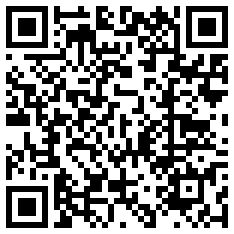
\includegraphics[width=2.7cm]{figures/qr/canonical.png}};
 \node at (0, -1.42) {\footnotesize\ttfamily\color{acgray} \paperhash};
 \node at (0, -2.12) {\scriptsize\ttfamily\color{acgray} papers.aesthetic.computer/keymaps-social-software-26-arxiv};
\end{scope}
\end{tikzpicture}}
\vspace{7pt}
{\scriptsize\raggedright\setlength{\parindent}{0pt}%
{\sffamily\bfseries\color{acgold!80!black} Historial de revisiones}\par\smallskip
\paperhistory\par}
\end{minipage}
\end{document}
